%; whizzy chapter
% -initex iniptex -latex platex -format platex -bibtex jbibtex -fmt fmt
% $B0J>e(B whizzytex $B$r;HMQ$9$k>l9g$N@_Dj!#(B


%     Tokyo Debian Meeting resources
%     Copyright (C) 2008 Junichi Uekawa
%     Copyright (C) 2008 Nobuhiro Iwamatsu

%     This program is free software; you can redistribute it and/or modify
%     it under the terms of the GNU General Public License as published by
%     the Free Software Foundation; either version 2 of the License, or
%     (at your option) any later version.

%     This program is distributed in the hope that it will be useful,
%     but WITHOUT ANY WARRANTY; without even the implied warranty of
%     MERCHANTABILITY or FITNESS FOR A PARTICULAR PURPOSE.  See the
%     GNU General Public License for more details.

%     You should have received a copy of the GNU General Public License
%     along with this program; if not, write to the Free Software
%     Foundation, Inc., 51 Franklin St, Fifth Floor, Boston, MA  02110-1301 USA

%  preview (shell-command (concat "evince " (replace-regexp-in-string "tex$" "pdf"(buffer-file-name)) "&"))
% $B2hA|%U%!%$%k$r=hM}$9$k$?$a$K$O(Bebb$B$rMxMQ$7$F(Bboundingbox$B$r:n@.!#(B
%(shell-command "cd image200804; ebb *.png")

%%$B$3$3$+$i%X%C%@3+;O!#(B

\documentclass[mingoth,a4paper]{jsarticle}
\usepackage{monthlyreport}
\usepackage[dvips]{xy}

% $BF|IU$rDj5A$9$k!"Kh7nJQ$o$j$^$9!#(B
\newcommand{\debmtgyear}{2008}
\newcommand{\debmtgmonth}{7}
\newcommand{\debmtgdate}{19}
\newcommand{\debmtgnumber}{42}

\begin{document}

\begin{titlepage}
\thispagestyle{empty}

% $B%?%$%H%k%Z!<%8(B:$BJT=8I,MW$JItJ,$O:G=i$N%^%/%m$KHt$P$9$3$H(B

\vspace*{-2cm}
$BBh(B\debmtgnumber{}$B2s(B $BEl5~%(%j%"(B Debian $BJY6/2q;qNA(B

\hspace*{-2.4cm}
\includegraphics[width=210mm]{image200801/2008title.eps}\\
\hfill{}\debmtgyear{}$BG/(B\debmtgmonth{}$B7n(B\debmtgdate{}$BF|(B

\end{titlepage}

\dancersection{Introduction}{$B>e@n(B $B=c0l(B}
 
 $B:#7n$N(BDebian$BJY6/2q$X$h$&$3$=!#$3$l$+$i(BDebian$B$N@$3&$K$"$7$rF'$_F~$l$k$H(B
 $B$$$&J}$b!"$9$G$K$I$C$W$j$H$D$+$C$F$$$k$H$$$&J}$b!"7n$K0l2s(BDebian$B$K$D$$(B
 $B$F8l$j$^$;$s$+!)(B

 Debian$BJY6/2q$NL\E*$O2<5-$G$9!#(B

\begin{itemize}
 \item \underline{Debian Developer} ($B3+H/<T(B)$B$N0i@.!#(B
 \item $BF|K\8l$G$N!V(B\underline{$B3+H/$K4X$9$k>pJs(B}$B!W$r@0M}$7$F$^$H$a!"%"%C%W%G!<%H$9$k!#(B
 \item \underline{$B>l(B}$B$NDs6!!#(B
 \begin{itemize}
  \item $BIaCJ$P$i$P$i$J>l=j$K$$$k?M!9$,(B face-to-face $B$G=P2q$($k>l$rDs6!(B
	$B$9$k!#(B
  \item Debian $B$N$?$a$K$J$k$3$H$r8l$k>l$rDs6!$9$k!#(B
  \item Debian$B$K$D$$$F8l$k>l$rDs6!$9$k!#(B
 \end{itemize}
\end{itemize}		

 Debian$B$NJY6/2q$H$$$&$3$H$G5f6KE*$K$O;22C<TA40w$,(BDebian Package$B$r$,$j$,$j(B
 $B$H:n$k%9!<%Q!<%O%C%+!<$K$J$C$?;Q$rLQA[$7$F$$$^$9!#>pJs$N6&M-!&3hMQ$rDL$7(B
 $B$F(B Debian$B$N:#8e$NG=F0E*$JE83+$X$NEZBf$H$7$F!"!V>l!W$H$7$F$N6u4V$rDs6!$9(B
 $B$k$N$,L\E*$G$9!#(B

$B0J>e$rL\E*$H$7$?!"(B2008 $BG/%"%8%'%s%@$G$9!'(B
\begin{enumerate}
 \item $B?7G/2q!V5$9g$rF~$l$k!W(B
 \item Open Source Conference Tokyo (3/1)
 \item $B%G!<%?$@$1$N%Q%C%1!<%8$r:n@.$7$F$_$k!"(B
       $B%i%$%;%s%9$N9M$(J}(B (David Smith)
 \item $B%P%$%J%j0l$D$N%Q%C%1!<%8$r:n@.$7$F$_$k(B ($B5HED(B@$BHD66(B)\\
       $B%P!<%8%g%s4IM}%D!<%k$r;H$$(BDebian$B%Q%C%1!<%8$r4IM}$9$k(B(git)\\
       $B%"%C%W%9%H%j!<%`$N07$$(B(svn/git/cvs)($B4d>>(B $B?.MN$5$s(B)
 \item $B%P%$%J%j$NJ,$1$?%Q%C%1!<%8$N:n@.!#(B($BA0ED$5$s(B)\\
       $B%P%$%J%j$NJ,$1J}$N9M$(J}!"%"%C%W%0%l!<%I$J$I$N1?MQ$H$+!#(B
 \item $B%Q%C%1!<%8:n@.(B(dpatch/debhelper$B$G:n@.$9$k%Q%C%1!<%8(B)($B>.NS576)$5$s(B)\\
       man $B$N=q$-J}(B(roff or docbook)($B$G$s$5$s(B)
       OSC 2008 Hokkaido
 \item $B%Q%C%1!<%8:n@.(B(kernel patch$B!"(Bkernel module)($B4d>>(B $B?.MN(B)
       Debconf$BH/I=N}=,!J>e@n$5$s!K(B

 \item Debconf $B%"%k%<%s%A%s!"6&M-%i%$%V%i%j%Q%C%1!<%8:n@.(B
       $B%3%_%C%/%^!<%1%C%H(B74

 \item Open Source Conference Tokyo/Fall$B!"(B
       $B%G!<%b%s7O$N%Q%C%1!<%8$N:n@.!"(Blatex$B!"(B emacs-lisp$B!"%U%)%s%H%Q%C%1!<%8(B
 \item $B%Q%C%1!<%8$N(B cross-compile $B$NJ}K!!"(Bamd64 $B>e$G(B i386 $B$N%Q%C%1!<%8$H(B
       $B$+!"(BOSC-Fall$BJs9p2q!"(BDebconf$BJs9p2q(B
 \item $B9q:]2=(B po-debconf / po$B2=(B / DDTP
 \item $BK:G/2q(B
\end{enumerate}


\newpage

\begin{minipage}[b]{0.2\hsize}
 \definecolor{titleback}{gray}{0.9}
 \colorbox{titleback}{\rotatebox{90}{\fontsize{80}{80} {\gt $B%G%S%"%sJY6/2q(B} }}
\end{minipage}
\begin{minipage}[b]{0.8\hsize}
\hrule
\vspace{2mm}
\hrule
\tableofcontents
\vspace{2mm}
\hrule
\end{minipage}

\dancersection{$B;vA02]Bj(B}{$B4d>>(B $B?.MN(B}

$B:#2s$N;vA02]Bj$O(B
\begin{enumerate}
 \item Debian $B$K<h$j9~$s$G$[$7$$(B Linux $B%+!<%M%k%Q%C%A!"(BLinux $B%I%i%$%P$r65$($F$/$@$5$$!#(B
 \item unstable $B$G%"%C%W%G!<%H$5$l$J$/$F:$$C$F$k(B Debian $B%Q%C%1!<%8!"(BBTS $B$KEPO?$5$l$F$$$k%P%0$N$&$A!"Aa$/D>$C$F$[$7$$%P%0$r5s$2$F$=$NM}M3$r65$($F$/$@$5$$!#(B
 \item {\bf $B$3$3$G3+:E$7$F$/$l$J$$$+$J$!(B} $B$H$$$&JY6/2q$N3+:ECO$r$=$NM}M3$H6&$K5s$2$F$/$@$5$$(B $B!J6a$$$+$i!"$@$1$O5Q2<!*!K!#(B
\end{enumerate}
$B$H$$$&$b$N$G$7$?!#(B
$B$=$N2]Bj$KBP$7$F2<5-$NFbMF$rDs=P$$$?$@$-$^$7$?!#(B

\subsection{$BNkLZ(B $B?rJ8(B $B$5$s(B}
$B$?$$$7$F<{MW$b$"$j$=$&$G$b$J$/!"7k9=IT0BDj$@$H$$$&OC$J$N$G!"8D?ME*$J<qL#$NLdBj$G$9$,!"(Bvlookback$B$H$$$&%+!<%M%k%b%8%e!<%k$,LLGr$$$N$GDI2C$G%$%s%9%H!<%k$G$-$k$H$&$l$7$$$G$9!#(Bvloopback$B$r;HMQ$9$k$H!"%S%G%*=PNO$K<j$r2C$($F2>A[E*$J%S%G%*F~NO%G%P%$%9$rDL$7$F%k!<%W%P%C%/$7$?$j$G$-!"$D$^$j(Bdv$BF~NO$r(Bv4l$B$KJQ49$7$?$j!"(Buvcvideo$B%G%P%$%9!J(Bv4l2$B!K$r(Bv4l$B$KJQ49$G$-$?$j$7$F(Bustream.tv$B$G$N%9%H%j!<%_%s%0$,;H$($k$h$&$K$J$C$?$j$7$^$9!#(B
$BDI2C%b%8%e!<%k$H$7$F(Bdeb$B%Q%C%1!<%8$GDI2C%$%s%9%H!<%k$G$-$k$N$J$i$P!":#2s$NJY6/2q$G3X$s$G;n$7$K<+J,MQ$N%Q%C%1!<%8$r:n@.$7$F$_$?$$$G$9!#(B

\subsection{$BA0ED!!9LJ?$5$s(B}

\begin{itemize}
\item Debian $B$K<h$j9~$s$G$[$7$$(B Linux $B%+!<%M%k%Q%C%A!"(BLinux $B%I%i%$%P$r65$($F$/$@$5$$!#(B
Debian$B$H$$$&$h$j$O!"(BLInux$B<+BN$KBP$7$F$J$s$G$9$,!"(Bbcm4328$B$,%5%]!<%H$5$l$k$H$&$l$7$$$G$9$M!#(BBroadcom$B$N@=IJ35MW$r8+$k$H(BLinux$B$O%5%]!<%H(BOS$B$K$O$J$C$F$$$k$b$N$N!"(BLinux
Wireless$B$N%5%$%H$r8+$k$H$^$@BP>]30(B\footnote{http://ja.broadcom.com/collateral/pb/4328-PB02-R.pdf}
$B$N$h$&$G$9!#@hF|!"(BNdiswrapper$B$r;H$C$F$h$&$d$/(BMacBook
Air$B$GL5@~(BLAN$B$rMxMQ$G$-$k$h$&$K$J$C$?$b$N$N!"9u(BMacBook$B$KHf$Y$k$H$I$&$b(BIP$B%"%I%l%9$N3d$jEv$F$,IT0BDj$G$9!J0lEY3d$jEv$F$5$l$k$H0BDj$9$k$s$G$9$,!K!#(BBB$B%b%P%$%k%]%$%s%H$G(BWEP$B$G@\B3$9$kJ,$K$O$^$C$?$/LdBjL5$+$C$?$N$G!"L5@~(BLAN$B%k!<%?$H$NAj@-$J5$$b$7$J$/$O$J$$$G$9$,!#(B\footnote{http://wireless.kernel.org/en/users/Drivers/b43\#unsupported}

Debian$B$K!"$H$$$&4QE@$G$O!"FCDj$N%Q%C%A$d%I%i%$%P$H$$$&$h$j$O!":G?7$N%Q%C%A$d%I%i%$%P!"%=%U%H%&%'%"$N(BSid$B$X$N<h$j9~$_$,$b$C$HAa$1$l$P$J$!!"$H;W$&$3$H$O$"$j$^$9!#(BUpstream$B$KHf$Y$k$HCY$/$J$k$N$O;EJ}$,L5$$$N$G$9$,!"$"$^$j$K$+$1N%$l$F$7$^$&$H!"<+J,$G(BUpstream$B$N:G?7HG$r;}$C$F$-$A$c$($P$$$$$+$H!"(BDebian$B%Q%C%1!<%8$O;H$o$:$K<+J,$G%S%k%I$7$F$7$^$&$N$G!#(B

\item {\bf $B$3$3$G3+:E$7$F$/$l$J$$$+$J$!(B} $B$H$$$&JY6/2q$N3+:ECO$r$=$NM}M3$H6&$K5s$2$F$/$@$5$$(B $B!J6a$$$+$i!"$@$1$O5Q2<!*!K!#(B

$B3d$H<j:"$JCMCJ$G<Z$j$i$l$=$&$J8uJd$r>e$2$F$*$-$^$9!#(B
\begin{itemize}
\item $B@23$6hL14[(B
\url{http://www.city.chuo.lg.jp/sisetugaido/syukaisisetu/syukaisisetu17/}
$B%$%s%?!<%M%C%H@\B34D6-$O$J$7!#%W%m%8%'%/%?!<$bL5$$$N$,%M%C%/$G$9!#(B

\item ITS$B7rJ]$N2q5D<<(B
$BH>F|<Z$j$i$l$k!"$H$$$&E@$G$O3d$H0B$$$G$9!#%W%m%8%'%/%?!<$O<Z$j$i$l$^$9!#(B
$B$^$?!"(BITS$B$N7rJ]AH9g0w$,$$$J$$$H<Z$j$i$l$^$;$s!#(B

\item $B;T%vC+2q5D<<(B
\url{http://www.its-kenpo.or.jp/restaurant/itigaya_kaigisitu/index.html}
$B>/?M?t(B(10$B?MDxEY(B)$B$N>l9g$O$^$!$^$!$+$b!#(B

\item $B;32&2q5D<<(B
\url{http://www.its-kenpo.or.jp/restaurant/sannou_kaigisitu/index.html}
$B$"$kDxEY?M?t$,$$$J$$$H%Z%$$G$-$^$;$s!#(B(50$B?M0J>e(B)

\item $BBg5WJ]2q5D<<(B
\url{http://www.its-kenpo.or.jp/restaurant/okubo_kaigisitu/index.html}
$BIt20$N<oN`(B($BDj0w(B)$B$O0lHVB?$$$G$9!#(B

\end{itemize}
\end{itemize}

\subsection{$B$d$^$M$5$s(B}
\begin{itemize}
\item BTS $B$KEPO?$5$l$F$$$k%P%0$N$&$A!"Aa$/D>$C$F$[$7$$%P%0$r5s$2$F$=$NM}M3$r65$($F$/$@$5$$!#(B

$B:G6a$O%P%0%&%)%C%A$7$F$J$$$N$G$J$s$H$b$`$:$+$7$$$G$9$,!"<+J,$,EPO?$7$F$k(B
ITP $B%P%0$r%/%m!<%:$7$?$$$J!<$H$OF|!9;W$C$F$$$^$9!#;W$C$F$k$@$1$G2?$b$7$F(B
$B$J$$$s$G$9$,!#$"$H$O(B l10n $B$J(B ja.po $B$OEPO?$7$F#1G/$H$+J|CV$5$l$k$HHa$7$$(B
$B5$J,$K$J$k$N$GAa$a$K$*4j$$$7$?$$=j$G$9!J:G6a$O(Bi18n$B$J(BNMU$B$G(Bfix$B$5$l$^$9$,!K!#(B

$B$D!<$+$M!"F0$+$M!<$H$+2?$+JQ$H$+$$$&$s$@$C$?$i!"(BBTS $B$KDI2C>pJs$@$;$h%4%k%!!*(B
$B$H$+;W$C$?$j$7$?$j$7$J$+$C$?$j$9$k:#F|$3$N:"!#(B
\end{itemize}

\subsection{$B$"$1$I$5$s(B}
\begin{itemize}
\item unstable $B$G%"%C%W%G!<%H$5$l$J$/$F:$$C$F$k(B Debian $B%Q%C%1!<%8!"(BBTS$B$KEPO?$5$l$F$$$k%P%0$N$&$A!"Aa$/D>$C$F$[$7$$%P%0$r5s$2$F$=$NM}M3$r65$($F$/$@$5$$!#(B

net-tools$B%Q%C%1!<%8$N$$$m$s$J%P%0(B
$BFC$K(Bnetstat$B%3%^%s%I$N(BIPv6$B%"%I%l%9$,@Z$jMn$H$5$l$k%P%0$O(B
lenny$B0J9_$G$NBP1~$,(B IPv4 $B%"%I%l%9$rI=<($9$k7A$K$J$C$F$$$F(B
$B$Q$C$H8+$?$@$1$GG!2?$K$b%@%a$J0u>]$K$J$C$F$7$^$&$N$G(B
upstream$B$r4^$a$F2?$H$+$7$FM_$7$$$H$3$m$G$9!#(B

$B$A$J$_$KB>$NK?%G%#%9%H%j%S%e!<%7%g%s$G$O(B
IPv6$B%"%I%l%9$,@5>o$KI=<($5$l$k$h$&$K$J$C$F$$$F(B
$B$H$F$bHa$7$+$C$?$j$7$^$9!#(B

$B$I$&$d$C$?$i%W%m%Q!<$J>u67$K$J$k$s$G$7$g$&$+!)(B
\end{itemize}

\subsection{$B0KF#(B $B90OB$5$s(B}
\begin{itemize}
\item unstable $B$G%"%C%W%G!<%H$5$l$J$/$F:$$C$F$k(B Debian $B%Q%C%1!<%8!"(BBTS$B$KEPO?$5$l$F$$$k%P%0$N$&$A!"Aa$/D>$C$F$[$7$$%P%0$r5s$2$F$=$NM}M3$r65$($F$/$@$5$$!#(B

$B%P%0$H$$$&$h$j$O!"(Bopen-vm-tools$B%Q%C%1!<%8$N=$@5$,0lCJMn$D$$$FM_$7$$$J$H;W$C$F$*$j$^$9!#(B
$BG.$$>uBV$H$$$&$3$H$b$"$j$^$9$,<+J,$b>oMQ$7$F$$$kJ*$3$=!"9W8%$G$-$k$h$&$K$J$j$?$$$H%Q%C%1!<%8$N=O@.$r%&%)%C%A$7$F$$$^$9!#(B
\end{itemize}

\subsection{$BBgGH!!@?$5$s(B}
\begin{itemize}
\item Debian $B$K<h$j9~$s$G$[$7$$(B Linux $B%+!<%M%k%Q%C%A!"(BLinux $B%I%i%$%P$r65$($F$/$@$5$$!#(B

$B@5D>$K?=$7>e$2$^$9!#%Q%C$H;W$$$D$/$b$N$,$"$j$^$;$s$G$7$?!#$?$@!"$3$N5!2q(B
$B$K!V(BLinux $B%I%i%$%P!W$H$+!V(Bdebian $B%I%i%$%P!W$H$+$G$0$0$C$F$_$^$7$?!#$=$7$?(B
$B$i(BThe Linux Foundation$B$,%G%P%$%9%I%i%$%P$N%*!<%W%s%=!<%92=$r@<L@$H$7$FH/I=(B
$B$7$F$$$?$j!!%0%i%U%#%C%/%\!<%I$N%I%i%$%P$J$I$N%W%m%W%i%$%(%?%j$J%=%U%H%&%'(B
$B%"$K4X$9$kLdBj$,:\$C$F$$$?$j$7$FJY6/$K$J$j$^$7$?!#(B
$BA0ED!!9LJ?$5$s$+$iJY6/2q$r>R2p$7$F$$$?$@$-$^$7$?!#(B
$B=i;22C$5$;$F$$$?$@$-$^$9!#(B
\end{itemize}

\subsection{$B;T@n(B $B7{?M$5$s(B}
\begin{itemize}
\item Debian$B$K<h$j9~$s$GM_$7$$(BLinux$B%+!<%M%k%Q%C%A(B

$B8D?ME*$J;v>p$J$N$G$9$,!"<+Bp%5!<%P$,(BMacBook$B$G$=$N%M%C%H(B 
$B%o!<%/%$%s%?!<%U%'%$%9$,(B
Marvell Yukon 88E805x$B$G!"(Bkernel$BI8=`$N(Bsky2$B%I%i%$%P(B 
$B$O$d$d5sF0$,2x$7$$$N$G!"(B
Marvell$BDs6!$N%I%i%$%P$r(Bdebian$B$N%Q%C%1!<%82=$7$F$"$k$HJX(B 
$BMx$G$9!#(B
$B<+J,$N5;=QNO$G$O(Bmake bzImage$B$9$iDL$i$J$+$C$?$N$G(B
$B$I$J$?$+5;=QNO$N$"$kJ}$,%Q%C%1!<%82=$7$F2<$5$k$HBgJQ4r$7$$$G$9!#(B
\end{itemize}

\subsection{$BK\>1$5$s(B}
\begin{itemize}
\item Debian $B$K<h$j9~$s$G$[$7$$(B Linux $B%+!<%M%k%Q%C%A!"(BLinux $B%I%i%$%P$r65$($F$/$@$5$$!#(B

$BFC$K;W$$$D$+$J$$$G$9!#(B

\item unstable $B$G%"%C%W%G!<%H$5$l$J$/$F:$$C$F$k(B Debian $B%Q%C%1!<%8!"(BBTS $B$KEPO?$5$l$F$$$k%P%0$N$&$A!"Aa$/D>$C$F$[$7$$%P%0$r5s$2$F$=$NM}M3$r65$($F$/$@$5$$!#(B

$B%"%C%W%G!<%H$5$l$J$/$F:$$C$F$$$k$H$$$&$o$1$G$O$"$j$^$;$s$,!":G6a(B
webmin$B$r;H$$$?$$$H;W$&$3$H$,$"$j!"$A$g$C$H;DG0$G$7$?!#(B


\item {\bf $B$3$3$G3+:E$7$F$/$l$J$$$+$J$!(B} $B$H$$$&JY6/2q$N3+:ECO$r$=$NM}M3$H6&$K5s$2$F$/$@$5$$(B $B!J6a$$$+$i!"$@$1$O5Q2<!*!K!#(B

$B0JA0$K$bOC$K>e$,$C$F$$$?!"29@t=I$O$I$&$G$7$g$&!#Lk$rE0$7$F8l$j9g(B
$B$&@h$K$J$K$+$,8+$($k$+$b$7$l$^$;$s!#(B
\end{itemize}

\subsection{$B_@Ln$5$s(B}
\begin{itemize}
\item Debian $B$K<h$j9~$s$G$[$7$$(B Linux $B%+!<%M%k%Q%C%A!"(BLinux $B%I%i%$%P$r65$($F$/$@$5$$!#(B

netfilter $B$N(B P-O-M patch $B$K4^$^$l$k(B ipset $B$H$$$&%b%8%e!<%k$r;HMQ$7$F$$(B
$B$^$9!#$J$+$J$+(B mainstream $B$KF~$C$F$/$l$J$$MM$J$N$G(B package $B$GMQ0U$7$F$*(B
$B$/$HJXMx$+$J!"$H;W$$$^$7$?!#(B

$B$b$&$R$H$D(B La Fonera $B$N%$%a!<%8$r?($k$N$K(B squashfs $B$b$"$k$H4r$7$$$+$J!"(B
mksquashfs $B$H$$$&%f!<%6%i%s%s%I%D!<%k$G$3$HB-$j$F$?$j$b$9$k$N$G$9$,(B\tt\symbol{94}\tt\symbol{94};
\end{itemize}

\subsection{$B@DLZ(B $B=$(B}
$B$^$"!"$+$J$jMxMQ<T$NA}$($F$$$k(BSCIM$B$G$9$,%Q%1!<%8%s%0$K;22C$5$l$F$$$k?M$,(B
$B$9$/$J$$$N$G!"$J$+$J$+%"%C%W%G!<%H$,DI$$$D$-$^$;$s!#(B

$B%a%$%s$N(BMING$B$5$s$OK;$7$$$N$G!"6(NO$7$F$/$l$k$+$?$$$^$;$s(B?$B;d$OC1$J$k(B
UPLOADER$B$G5;=QE*$K$3$l$OFq$7$$$N$G!"$$$$?MC5$7$F$$$^$9!#(B

$B$"!<!"3+:E>l=j$G$9$,!"El9)Bg$ND9DEED%-%c%s%Q%9$J$I$@$l$+3X@8$5$s$,$$$=$&(B
$B$J$N$K$J$<$J$$$N$+$J!<$H$$$D$b;W$C$F$$$^$9!#(B

\subsection{$BF#Bt(B $BM}Ao(B $B$5$s(B}
\begin{itemize}
\item {\bf $B$3$3$G3+:E$7$F$/$l$J$$$+$J$!(B} $B$H$$$&JY6/2q$N3+:ECO$H$=$NM}M3(B

$B3+:ECO!'3X9;!J9b9;!&Bg3X$J$I!K(B
$BM}M3!'(B
$B0l8@$G8@$&$H!"3X@8$K6=L#$r;}$C$FM_$7$$$+$i$G$9!#(B
Debian$B$K?($l$k$N$KG/Np$O4X78$J$$$H;W$&$1$l$I!"(B
$B<c$$$&$A$K(BDebian$B$K?($l$k$N$b0-$/$J$$$H;W$$$^$9!#(B
$B3X9;$H$$$&>l=j$d3X@8$H$$$&N)>l$G$O!"(B
$B:#$N$H$3$m(BLinux$B$N$h$&$J%U%j!<$J(BOS$B$K?($l$k5!2q$O(B
$BB?$/$J$$$N$,;DG0$G$9!J<R2q$K=P$F$b?($l$k5!2q$OB?$/$J$$$1$I!K!#(B
$B$H$K$+$/!"$^$@CN$i$J$$?M$,6=L#$r;}$C$F$/$l$=$&$J!"(B
$B$=$&$$$&>l=j$G3+:E$9$k$N$b$$$$$s$8$c$J$$$+$J!"$H;W$$$^$7$?!#(B
\end{itemize}

\subsection{$B4d>>(B $B?.MN(B}
\begin{itemize}
\item Debian $B$K<h$j9~$s$G$[$7$$(B Linux $B%+!<%M%k%Q%C%A!"(BLinux $B%I%i%$%P$r65$($F$/$@$5$$!#(B

$B:#2s$N;qNA:n@.$N$D$$$G$K:n$j$^$7$?!#FbMF$OH/I=$r;2>H!#(B

\item unstable $B$G%"%C%W%G!<%H$5$l$J$/$F:$$C$F$k(B Debian $B%Q%C%1!<%8!"(BBTS $B$KEPO?$5$l$F$$$k%P%0$N$&$A!"Aa$/D>$C$F$[$7$$%P%0$r5s$2$F$=$NM}M3$r65$($F$/$@$5$$!#(B

kernel-package $B4X78$N%P%0$J$I!#%a%s%F%J(B(Manoj)$B%5%\%j5$L#$G$9$M!#:$$j$^$7$?$M!#(B
libflash $B$NIT6q9g$,D>$C$F$J$$$N$r$J$s$H$+$7$F$[$7$$!#(B

\item {\bf $B$3$3$G3+:E$7$F$/$l$J$$$+$J$!(B} $B$H$$$&JY6/2q$N3+:ECO$r$=$NM}M3$H6&$K5s$2$F$/$@$5$$(B $B!J6a$$$+$i!"$@$1$O5Q2<!*!K!#(B

$B@hF|!"El5~EE5!Bg3X$5$s$K9T$C$F!"%3%i%\$G$-$J$$$+AjCL$7$F$-$^$7$?!#3X@8$5$s$K6=L#$r;}$?$;$k$K$O$I$&$7$?$i$$$$$G$9$+$M!#(B
$B$"$H$O29@t$r(B8$B7n$K4k2hCf$G$9!#(B

\end{itemize}

%%% trivia quiz
\dancersection{Debian Trivia Quiz}{$B>.NS(B $B576)(B}

$B$H$3$m$G!"$_$J$5$s(B Debian $B4XO"$NOCBj$K$*$$$D$$$F$$$^$9$+!)(BDebian$B4XO"$NOC(B
$BBj$O%a!<%j%s%0%j%9%H$r$h$s$G$$$k$HDI@W$G$-$^$9!#$?$@$h$s$G$$$k$@$1$G$O$O(B
$B$j$"$$$,$J$$$N$G!"M}2rEY$N%F%9%H$r$7$^$9!#FC$K0l?M$@$1$G$O0UL#$,$o$+$i$J(B
$B$$$H$3$m$b$"$k$+$bCN$l$^$;$s!#$_$s$J$G0l=o$KFI$s$G$_$^$7$g$&!#(B

$B:#2s$N=PBjHO0O$O(B\url{debian-devel-announce@lists.deban.org} $B$KEj9F$5$l$?(B
$BFbMF$H(BDebian Project News$B$+$i$G$9!#(B
% $B=PBjHO0O(B: http://lists.debian.org/debian-devel-announce/2008/06/msg00004.html $B!A(B http://lists.debian.org/debian-devel-announce/2008/07/msg00004.html
\begin{multicols}{2}
 \subsection{debian-devel-announce}
 \url{debian-devel-announce@lists.deban.org}$B$X$NEj9FFbMF$+$i$G$9!#(B
 
 \santaku
 {Perl 5.10$B$N%P%0$G$I$N$h$&$JLdBj$,H/@8$7$?(B?}
 {Ruby$B$H(BPython$B$G=q$+$l$?%"%W%j%1!<%7%g%s$d%i%$%V%i%j$,%$%s%9%H!<%k$G$-$J$$(B}
 {$B%$%s%9%H!<%k$5$l$?%U%!%$%k$N%Q!<%_%C%7%g%s$,(B0777$B$K$J$k(B}
 {$BFCDj$NL>A0$N%U%!%$%k$,%$%s%9%H!<%k$G$-$J$$(B}
 {B}% File::Path::rmtree$B$,%D%j!<:o=|A0$K%Q!<%_%C%7%g%s$r(B0777$B$K$7!"$=$l$,(Bsymlink$B$N%j%s%/85$K$bEAGE$9$k$h$&$K$J$C$F$$$?$N$,860x!#(Bpostinst$B$G8F$S=P$5$l$k(Bdebsign$B$,%D%j!<$N(Bsymlink$B$r:n@.$7$F%O%C%7%e$r7W;;$7$?8e!"$3$N4X?t$r;H$C$F(Bsymlink$B$r:o=|$7$F$$$k$N$G!"%$%s%9%H!<%k8e$K%U%!%$%k$N%Q!<%_%C%7%g%s$,=q$-49$($i$l$kLdBj$KH/E8$7$?(B
 
 \santaku
 {Debian$B%W%m%8%'%/%HFb$N%A!<%`$K4X$9$kD4::$GH=L@$7$?!VM=A[30$N%A!<%`!W$G$J$$$b$N$O(B?}% $BD4::$O(BDPL$B$N(BSteve McIntyre$B$,9T$C$F$$$k(B
 {$B<B:]$KF0$$$F$$$k$N$O(B1$B?M$@$1$H$$$&%A!<%`(B}
 {$BC/$,:n6H$9$k$+Kh2s$8$c$s$1$s$G7h$a$F$$$k%A!<%`(B}
 {$B$*4j$$$d$"$j$,$H$&$G$O$J$/6<Gw$GF0$$$F$$$k%A!<%`(B}
 {B}
 
 \santaku
 {wxwidgets2.8$B$,%"%C%W%m!<%I$5$l$?$,!"D9$$$3$H(Bwxwidgets2.6$B$N;~Be$,B3$$$F$$$?!#$=$NM}M3$O(B?}
 {$B%Q%C%1!<%8%a%s%F%J$,J]<iE*$G!"(B2.8$B$N;HMQ$KBP$7$FHs@Q6KE*$@$C$?(B}
 {$B%"%C%W%m!<%I$7$?$H$3$m$G$I$&$;C/$b;H$C$F$/$l$J$$$H%Q%C%1!<%8%a%s%F%J$,;W$C$?(B}
 {$B%Q%C%1!<%8%a%s%F%J$,B?K;$G:n6H;~4V$,$H$l$J$+$C$?(B}
 {A}% lenny$B$G$O(B2.6$B$r%G%U%)%k%H$H$7!"(B2.6$B$GF0$+$J$$$b$N$@$1(B2.8$B$r;H$C$F$[$7$$!"$H$N$3$H(B
 
 \santaku
 {Frans Pop$B$N<-G$$K$h$C$F!"?7$?$J<9I.<T$,5a$a$i$l$k$h$&$K$J$C$?$b$N$H$O(B?}
 {$B%j%j!<%9%N!<%H(B}
 {Debian Project Blog}% Debian Project$B8x<0$N(Bblog
 {DEB NOTE}% $BL>A0$,=q$+$l$?3+H/<T$r6/@)E*$K%3%_%e%K%F%#$+$iDI$$=P$9%N!<%H(B
 {A}
 
 \subsection{Debian Project News 2008$BG/(B05$B9f(B}
 \url{http://www.debian.org/News/weekly/2008/05/}
 $B$K$"$k(B6$B7n(B23$BF|HG$G$9!#(B
 
 \santaku
 {debian/rules$B$N(Bget-orig-source$B%?!<%2%C%H$O2?$r5-=R$9$k$?$a$N$b$N$+(B?}
 {$B!V%*%j%8!{J[Ev!W$GJ[Ev$K%=!<%9$r$D$1$F$b$i$&J}K!(B}
 {upstream$B$+$i%M%C%H%o!<%/7PM3$G%=!<%9%3!<%I$r<hF@$7$F8=:_$N%=!<%9%3!<%I$HCV$-49$($kJ}K!(B}
 {upstream$B$+$i%M%C%H%o!<%/7PM3$G:G?7$N(B.orig.tar.gz$B%U%!%$%k$r<hF@$9$kJ}K!(B}
 {C}% $B$"$^$j=q$+$l$k$3$H$N$J$$%?!<%2%C%H$@$,!"(Bskkdic$B$G$O(BCVS$B7PM3$G<hF@$9$k$h$&@_Dj$7$F$$$k(B
 
 \santaku
 {$B%j%j!<%9%4!<%k$K4X$9$k(BPeter Eisentraut$B$N0U8+$O(B?}
 {$B%j%j!<%9%4!<%k$J$s$F=jA'0lIt$N3+H/<T$N3Z$7$_$K2a$.$J$$(B}
 {Debian$B$N5!G=$N<BAu$K4X$9$k%j%j!<%9%4!<%k$O%j%j!<%98e$K%]%j%7!<$X$HJQ$($k$Y$-$@(B}
 {$B%j%j!<%9$J$s$F>~$j$G$9!#0N$$?M$K$O$=$l$,$o$+$i$s$N$G$9$h(B}
 {B}
 
 \santaku
 {William Pitcock$B$,:o=|$rDs0F$7$?%V!<%H%m!<%@%Q%C%1!<%8$O(B?}
 {grub}
 {lilo}
 {yaboot}
 {B}% $B4JC1$K$OD>$;$J$$(Bgrave$B$J%P%0$,$"$k(B
 
 \santaku
 {Debian weather$B$H$O$I$s$J%5!<%S%9$+(B?}
 {$BFCDj%"!<%-%F%/%A%c$N%"!<%+%$%V$N>uBV$rMWLs$7$FI=<($9$k(B}% $B$=$NI=<($KE75$$N5-9f$r;HMQ$7$F$$$k(B
 {Debian$B4XO"%[%9%H$,CV$+$l$F$$$k@$3&3FCO$NE75$$rI=<($9$k(B}% worldwide$B$GF/$$$F$$$k$H$$$&0U<1$r9b$a$k(B
 {$B%a!<%j%s%0%j%9%H$NN.NL$+$i@$3&3FCO$NE75$$r?dB,$7$FI=<($9$k(B}% $B$3$NCO0h$+$i$N%a!<%k$,B?$$$+$i$3$NCO0h$O1+$@$J!"$H$+(B
 {A}
 
 \subsection{Debian Project News 2008$BG/(B06$B9f(B}
 \url{http://www.debian.org/News/weekly/2008/06/}
 $B$K$"$k(B7$B7n(B7$BF|HG$G$9!#(B
 
 \santaku
 {Debian 15$B<~G/$O$$$D$+(B?}
 {$B<!2s$NEl5~%(%j%"(BDebian$BJY6/2q3+:EM=DjF|$G$"$k(B8$B7n(B16$BF|(B}
 {$BK\F|(B7$B7n(B19$BF|(B}
 {$B5c$/;R$bL[$k(B7$B7n(B9$BF|(B}
 {A}
 
 \santaku
 {Debian$B$N%a%K%e!<(B (.menu$B%U%!%$%k(B) $B$H%G%9%/%H%C%W4D6-$N%a%K%e!<(B (.desktop$B%U%!%$%k(B) $B$K4X$9$k5DO@$O$I$N$h$&$J7kO@$KMn$ACe$$$?$+(B?}
 {freedesktop.org$B$N(B.desktop$B%U%!%$%k$r(BDebian$B$K9g$&$h$&3HD%$7$F;H$C$F$$$3$&(B}
 {freedesktop.org$B$N(B.desktop$B%U%!%$%k$K$OITJX$JE@$,$"$k$N$G!"F/$-$+$1$F=$@5$7$F$b$i$*$&(B}
 {freedesktop.org$B$N(B.desktop$B%U%!%$%k$O;H$($J$$$N$G(BDebian$B$N(B.menu$B%U%!%$%k$r;H$o$;$h$&(B}
 {A}% .desktop$B%a%K%e!<$O%f!<%6%S%j%F%#$rL\E*$H$9$k$b$N$GC10l3,AX(B ($B%5%V%+%F%4%j$J$7(B) $B$J$N$KBP$7!"(BDebian$B$N%a%K%e!<$O40A4@-$rL\E*$H$9$k$b$N$G3,AX$r?<$/7!$C$F$$$k!#$A$J$_$K(B.menu$B$KHf$Y$F(B.desktop$B$N$[$&$,$$$$$H$$$&?M$O$+$J$jB?$=$&(B
 
 \santaku
 {6$B7nKv$K=i$a$FCB@8$7$?(BDebian$B3+H/<TF1;N$NIWIX$H$O(B?}
 {Junichi Uekawa$B$H(BKenshi Muto}
 {Meike Reichle$B$H(BAlexander Schmehl}
 {Debra Murdock$B$H(BIan Murdock}% $B<B$O(BDebra$B$5$s$,(BDD$B$K$J$j:#99$J$,$i7k:'!"$H$+(B
 {B}
 
 \santaku
 {$B7k:'$7$?Fs?M$K$D$$$F=R$Y$?0J2<$N;v9`$N$&$A!"@5$7$$$b$N$O(B?}
 {$B:G=i$NB#$jJ*(B: DebConf5$B$NEZ;:(B}% $B6qBNE*$K$O(BDebConf5$B$N(BT$B%7%c%D$H%U%#%s%i%s%I$N%A%g%3%l!<%H(B
 {$BHkL)$N0&$N8r49<jCJ(B: wiki.debian.org}% planet.d.o$B$G8r49$7$F$$$?$iC/$+$K=q$-49$($i$l$?(B
 {$B:'Ls$N8x<0H/I=<jCJ(B: lists.debian.org}% planet.d.o$B$GH/I=$7$?$iL>A0$r=q$-49$($i$l$?(B
 {A}

\end{multicols}
\dancersection{$B:G6a$N(BDebian$B4XO"$N%_!<%F%#%s%0Js9p(B}{$B4d>>(B $B?.MN(B}
\subsection{$BEl5~%(%j%"(BDebian$BJY6/2q(B41$B2sL\Js9p(B}
6$B7n$NBh(B41$B2sEl5~%(%j%"(BDebian$BJY6/2q$r<B;\$7$^$7$?!#(B $B:#2s$N;22C<T$O(B $B$"$1$I$5$s!"A0ED$5$s!">.NS576)$5$s!"5HED!wHD66$5$s!";3K\(B $B9@G7$5$s!"(B $B;3K\Bv$5$s!"F#BtM}Ao$5$s!"F|HfLn(B $B7<$5$s!"NkLZ(B $BK.CK$5$s!"4d>>$N(B10$B?M$G$7$?!#(B

\begin{itemize}
    \item $B$^$::G=i$K:G6a$N%_!<%F%#%s%0$NJs9p$r9T$$$^$7$?!#(B
    \item $B:#2s$N%/%$%:$O4d>>$,=PBj$7$^$7$?!#A4Ld@52r<T$O$$$^$;$s$G$7$?!#;w$?$h$&$JEz$($,B?$/!"2sEz<T$O:$$C$F$$$^$7$?!#(B
    \item $B;vA02]Bj$r>R2p$7$^$7$?!#(B AIX$B$N%m%0%7%9%F%`$HDs6!$5$l$F$$$k(B errpt $B%3%^%s%I$,$+$J$j$$$1$F$$$k$h$&$G$9!#<B:]$K<B5!$r?($C$F$I$s$J46$8$J$N$+8+$F$_$?$$$G$9!#$"$H!"(Bhinemos $B$NOC$,=P$^$7$?!#(BDebian$B$G;H$$$?$$J}$,B?$$$h$&$G$9$,!"(BJava $B$G<BAu$5$l$F$*$j!"MW5a$9$k%^%7%s%9%Z%C%/$b9b$$$?$a!"%Q%C%1!<%8%s%0$H%F%9%H$NF;$N$j$O7c$7$/1s$$5$$,$7$^$7$?!#(B
    \item 2008$BG/$N%F!<%^$O(BDEB$B%Q%C%1!<%8$N3+H/!&4IM}$K4XO"$7$?FbMF$G$9$,!"(B 4$B2sL\$N%F!<%^$H$7$F>.NS$5$s$,(Bdebhelper$B$r;H$C$?%Q%C%1!<%8%s%0J}K!$K$D$$$F>R2p$7$^$7$?!#(Bdebhelper $B$r;H$o$J$$%Q%C%1!<%8%s%0J}K!$+$i!"(Bdebhelper $B$r;H$C$?J}K!!"(Bcdbs $B$r;H$C$?J}K!$r$$$&N.$l$GOC$7$F$/$l$?$N$G!"(Bdebhelper$B$H(Bcdbs$B$N$"$j$,$?$5$,J,$+$j$^$7$?!#(B
    \item $B:G6a$N(B kFreeBSD, nexenta, Hurd, SuperH, eeepc $B$K$D$$$F>R2p$7$F=*N;$7$^$7$?!#(B
    \item $B1#$75e$@$C$?;3K\$5$s$N(B Hurd $B%f!<%6!<$rA}$d$92q$NH/I=$,$G$-$^$;$s$G$7$?!#(B
    \item $B:#2s$bJY6/2q$N4V0c$($F$7$^$C$??M$,$*$i$l$^$7$?!#3+:E>l=j$OKh2s%A%'%C%/$9$k$h$&$K$7$^$7$g$&!#(B
    \item $BJY6/2q$N$"$H!"5o<r20$5$D$-$G1c2q$r$7$^$7$?!#(BDebian $B$0$k$0$k%+%C%F%#%s%0%9%F%C%+!<$rHNGd$7$F$_$?$H$3$m!"$J$+$J$+$N9%I>$V$j$G$7$?!#$5$C$=$/(BPC$B$KE=$C$F$$$k?M$b$*$j!"BgK~B-$N$h$&$G$9!#%9%F%C%+!<$,M_$7$$?M$O;d$KO"Mm$r$/$@$5$$!#(B 
\end{itemize}

% (query-replace-regexp "<.*?>" "")
% (query-replace-regexp "^[	 ]\+" "")


\subsection{eeePC Developers Conference day 1}

$B7P:QIt9)6H6I!#(B
$BEPO?$7$?$iL5NA$G;22C$G$-$k%+%s%U%!%l%s%9!#(B
$B9V1i<T$,A40w%9!<%D$r$-$F$$$^$9$,!"Mh>l$7$F$$$kJ}!9$OIaCJCe$G$9!#(B
$B%+%a%i$N%U%i%C%7%e$NNL$+$i$OCmL\EY$,;G$($^$9!#(B
$B7HBSEEOC$NCe?.2;$,$J$j$[$&$@$$$G$9!#(B

$B3+;O$N%*!<%W%K%s%0$OB?>/$*$/$l$^$7$?$,$[$\K~0w$G3+;O$7$^$7$?!#(B
$B8eH>$K$J$k$HH>J,$/$i$$$NKd$^$jJ}$K$J$j$^$7$?!#(B

$B$_$J$5$^(BeeePC$B$G%W%l%<%s$7$F$$$^$9$,!"(B
$B%W%m%8%'%/%?!<$,F14|$H$l$F$$$J$$46$8$G!"A4BN$,$&$D$C$F$$$^$;$s!#(B

$B30$O=k$/!"2q>l$,4($$$N$@$1$I!"$_$s$J$J$l$F$$$k$b$N$G%8%c%s%Q!<Ce$F$^$9!#(B

5$B7n(B8$BF|$K(B1$BF|L\$,3+:E$5$l$^$7$?!#(B

\begin{tabular}{|c|p{18em}|c|}
09$B!'(B00 ~ 09$B!'(B30 & 	 Register & \\
09$B!'(B30 ~ 09$B!'(B45 &	Opening Remarks & \\
09$B!'(B45 ~ 10$B!'(B20 &	Keynote Speech Keynote Speech -- EeePC Software Platform Business Model &	ASUS | Ellis Wang\\
10$B!'(B20 ~ 10$B!'(B50 &	EeePC Application Demo Show &	ASUS  Patrick Chou\\
10$B!'(B50 ~ 11$B!'(B00 &	Tea Break &\\
11$B!'(B00 ~ 12$B!'(B20 &	EeePC SDK Announcement and Demo &	ASUS\\
12$B!'(B20 ~ 13$B!'(B40 &	Lunch &\\
13$B!'(B40 ~ 14$B!'(B30 &	The rule of game to stand on the shoulders of giant 	&Florence T.M. Ko, OSSF\\
14$B!'(B30 ~ 15$B!'(B10 &	Developing with pyGTK in EeePC 	&TsungWei Hu, OSSF\\
15$B!'(B10 ~ 15$B!'(B30 &	Tea Break &\\
15$B!'(B30 ~ 16$B!'(B10 &	Developing with pyQT in EeePC 	&Gary Lee\\
16$B!'(B10 ~ 16$B!'(B50 &	Firefox Platform Application Programming 	&Thinker\\
16$B!'(B50 ~ 17$B!'(B30 &	Google Gears Programming 	&Tzeng Chien-Ming\\
17$B!'(B30 ~ 17$B!'(B40 &	Software Vendor Panel Discussion 	&ASUS\\
\end{tabular}


\subsubsection{$B3+2q$N$40';"(B}

eeePC SDK $B$NH/I=(B

Open Source Development

\subsubsection{$B3+2q$N$40';"(B2}

$B2?$+$NOC!"$^$C$?$/$o$+$i$:!#(B

\subsubsection{Announcement of eeePC SDK, Dev tools and Community}

ASUS$B$N(BEllis Wang$B;a$,H/I=$7$^$7$?!#(B
eeePC$B$G%W%l%<%s$7$F$$$^$9!#(B
$B%*!<%W%s%=!<%9$N%G%Y%m%C%Q!<$N?M$?$A$K$G$-$k$@$1;22C$7$F$[$7$$$H$$$&5$;}(B
$B$A$,EA$o$C$F$-$^$9!#(B
$B1Q8l$N%W%l%<%s$G!"Cf9q8l$GH/I=$7$F$$$^$9!#(B

$B:G=i$K3+2q$N0';"$r$7$?$($i$$$R$H$K$J$<$+(BeeePC$B$rB#Dh$7$F$$$^$9!#(B

Linux $B$G!"%3%_%e%K%F%#!<$K$D$$$F$J$s$?$i!#(B

ISV$B$H%3%_%e%K%F%#!<(B

SDK$B$NOC!#(B

ASUS$B$H(BeeePC$B$N%=!<%9%3!<%I$,(B
$B%D!<%k%@%&%s%m!<%I$G$-$k$h$M!#(B

$B%*!<%W%s%=!<%9%3%_%e%K%F%#!<$,(BeeePC$B$r;Y1g$7$F$$$k!#(B

Linux $B$K$+$.$i$:!"(BDebian, KDE $B$J$I$,$"$k!#(B

Microsoft$B$N(BUI$B$KHf$Y$F!"(BUI$B$NJQ99$,4JC1$H8@$C$F$$$k$h$&$J5$$,$9$k!#(B

Linux $B$NAG@2$i$7$5$K$D$$$F!#(B
EeePC:

\begin{itemize}
 \item easy -- to learn, work and play
 \item excellent -- on the go
 \item excellent -- internet experience
\end{itemize}

$B%$%s%F%0%l!<%7%g%s$9$k$3$H$NBg@Z$5!#(B
contribution $B$r9T$&!#(B

$BHFMQ$N%D!<%k$N%=!<%9$rAH$_9g$o$;$F:n$j>e$2$k!#(B

$B%*!<%W%s%=!<%9$O6&M-$9$k$3$H$,Bg@Z$G$"$j!#(B
IP$B$NOC!#(B
[share]

warranty $B$NOC(B?

reuse$B$NOC!#(B


EeePC SDK$B$H$O(B?

$B%^%K%e%"%k$NL\<!$r2hLL$K$&$D$9!#(B
EeePC$B$N%Q%C%1!<%8$O(BDebian$B%Q%C%1!<%8$@$h!#(B

$B%Q%C%1!<%8$N%F%9%H$O(B?VMware$B$r$D$+$*$&!#(B

eeePC$B$O3+H/<T!&(BASUS$B!&%f!<%6!&(BCC$B%G%8%?%k%3%s%F%s%H$r$D$J$0$?$a$N%V%j%C%8$@!#(B

$BL5@~$H$+(BCPU$B$H$+%+!<%M%k$H$+$O(BASUS$B$,$d$k$@$m(B?

GPL$B$@$m!"$H$+!#(B

Debian$B$N%Q%C%1!<%8$H$+$rDs6!$9$k!#(B

$B%P!<%A%+%k$G(BNo1$B$rL\;X$9!#(B
$B%F%l%3%`$H650iL\E*$K!#(B

partner $B$N%l%Y%k$,$"$k!#(B

$B%7%9%F%`$H(BOS$B$N%Q!<%H%J!<$O0lHV>/$J$$$,%$%s%F%0%l!<%7%g%s$NEY9g$$$,9b$$!#(B

SDK$B:n$C$?$N$G%*!<%W%s%=!<%9%G%Y%m%C%Q!<$?$A$K%G%Y%m%C%W%a%s%H%3%_%e%K%F%#!<(B
$B$r$D$/$k$3$H$,$G$-$k$@$m(B?
$B%3%^!<%7%c%k%Y%s%@!<$b%D!<%k$,=<<B$7$F$$$FK~B-$9$k$K$A$,$$$J$$!#(B
$B%*!<%W%s%=!<%9$N5;=Q<T$b$h$/CN$C$F$$$k5;=Q$G$&$l$7$$$K0c$$$J$$!#(B

Eclipse $B$H(B Qt4 $B$N3+H/%D!<%k%-%C%H$,$O$$$C$F$$$k$<!#(B

$B3+H/%W%m%;%9$N(B
Phase$B$OFs<oN`$"$k!#(B
$B<B5!$H(BVMware$B$@!#(B
$B%U%'!<%:%$!<$H%U%'!<%:%"%k!#(B


$B%F%9%H$N>.5;!#(B
$B2hLL%5%$%:$H$+A4It;n$7$F$*$/$N$,$h$$$G$9!#(B

$B%G%9%/%H%C%W$HHf$Y$k$H0lIt0c$$$^$9!#(B
ASUS desktop$B$G!"%f!<%6%"%+%&%s%H$,0l$D$7$+$J$$$h!#(B
$B$^$?!"(Binit$B$O%_%K%^%k$G$9!#(B

howto 

$B2hLL>.$5$$!#(B
Flash$B$O(B10$BK|2s=q$-9~$`$H(B wear out $B$9$k$N$G$G$-$k$@$1=q$-9~$_$7$J$$!#(B

eeePC$B%"%W%j%1!<%7%g%s$N0\?"$O4JC1$h!#(B
Java$B$bF0$/!#(BPicasa$B$O(BWine$B$GF0$$$F$$$k!#(B
(Linux$B$N@bL@$r$7$F$$$k5$$,$9$k!#(B)

Adobe flash $B$O%5%]!<%H$9$k$1$I(BAIR$B$O%@%a$@$M(B(?)$B!#(B


$B$H!"=*$o$C$?$i?M$,A{A3$H$7$O$8$a$?!#(B
$B5Y7F;~4V3+;O!#%9%J%C%/$H%3!<%R!<$,Ds6!$5$l$^$7$?!#(B

\subsubsection{$B650iMQ$N%"%W%j%1!<%7%g%s(B?}

$B3t<0<h0z%D!<%k(B

$BH/2;$N=P$k<-=q(B

$B%+%i%*%1$_$?$$$J!"2;3Z$,N.$l$J$,$i2N;l$HLu8l$N=P$k%D!<%k!#(B

ASUS MeBook

MeReader MeSong


$BK\$rGc$&$3$H$,$G$-$k!#(B

$B%i%C%WIw$NCf9q8l2qOC!#(BIQChinese$B!#(B
PinYin$B$NJY6/$5$;$F$/$l$k!#(B


$B2;@<@)8f$N%D!<%k!#(BSkype$B$r@<$G5/F0$G$-$k(B?

$B0l%Z!<%8$a$/$k$H2;@<$G;X<($r=P$7$F%W%l%<%s$r@)8f$7$F$$$k!#(B

\subsection{Introduction to eeePC SDK}

Chih Wei Huang

$B@V$A$c$s$G$b$D$+$($k$/$i$$%7%s%W%k$@$h!"(B
$B$H@V$A$c$s$N<L??$r8+$;$F(Bice-break$B!#(B

eeePC900 $B$O(B2008$BG/(B4$B7n!"(B8.9'' $B%7%j!<%:$H$7$FEP>l!#(B

eeePC$B$O(BDebian$B%Y!<%9$G$9!#(B
$B%*!<%W%s%=!<%9$G$9$h!#(B

Xandros open circulation edition $B$H$$$&$N$r$D$+$C$F$^$9!#(B
$B3+H/4D6-$O(BEclipse $B$G$9!#(B

Qt4$B$O:#$O(BNokia$B$N(BTrolltech$B$,3+H/!#(B


$BI8=`$N(B.deb$B%Q%C%1!<%8$r;H$C$F$$$k!#(B
SDK$B$H$7$F!"(Bdebian policy manual, new maintainer guide$B$H$+$,>R2p!#(B
$B%(%-%9%Q!<%H$,$?$/$5$s$$$k$h!"$H!#(B

$B%G%9%/%H%C%W$K%"%$%3%s$rDI2C$9$kJ}K!$O4JC1$@$h!#(B
XML$B%U%!%$%k$r:n@.$9$l$P$h$$!#(B

\url{http://sourceforge.net/projects/eeecommunity/}
$B$K(BVMware $B$N%$%a!<%8$O$"$k$+$i8+$F$M!#(B
ISO$B$r(Bvmware-convert $B%3%^%s%I$GJQ49$7$?$iMxMQ$G$-$k$h!#(B
eeePC 701 $B$N%$%a!<%8$J$I$,$"$k!#(B

i18n/l10n$B$O!"(BQt $B$H(B gettext $B$,$"$k$h!#(B
Qt $B$O(B tr().
lupdate$B$H$+;H$&!#(B
gettext$B$O(B \verb!_()!$B$G!#(B


Eclipse$B$N(BQt$BMQ$N3+H/%D!<%k$,$"$k$h!#(B
Qt Designer $B$,(B Eclipse$BFbIt$GF0:n$7$^$9!#(B


\subsubsection{The rule of game to stand on the shoulders of giant}

GPL$B$N<vG{$r2sHr$9$kJ}K!$K$D$$$F!#(B

FOSS$B$N:[H=0F7o$N>R2p!#(B

Busybox $B:[H=$J$I!#(B

Creative Commons $B$N$9$9$a$H$+!#(B

$B<ALd$O!"(BGPL $B$N7Q>5$rHrLH$9$kJ}K!$K$D$$$F!#(B
dynamic linker $B$H(B static link $B$NOC$r$7$F$$$?$h$&$J5$$,$9$k!#(B

\subsubsection{Developing with pyGTK in EeePC}

??
Open Source Software Foundry Introduction $B$+$b(B?

$B<+M3$H$O!#(B

OSSF$B$NOC(B

Python$B$r;H$&$3$H$K$D$$$F!#(B
python $B$NJ8K!$K$D$$$F!#%$%s%G%s%H=EMW$H$+(B

Gtk $B$H$+!#(B

\subsubsection{Developing with pyQT in EeePC}

PyQt$B$N;HMQJ}K!$K$D$$$F$N>R2p!#(B

\subsubsection{Firefox Platform Application Programming}

$B%O%C%+!<A3$H$7$?!V(Bthinker$B!W$K$h$k(B firefox $B%W%i%C%H%U%)!<%`%"%W%j%1!<%7%g%s%W%m%0%i%_%s%0(B
$B$N>R2p!#(B

$B!V(BOK$B!W$H$7$+I=<($7$J$$(B mozilla $B%"%W%j%1!<%7%g%s$NNc$N>R2p!#(BXUL$B!#(B

$B;~4V%*!<%P!<$@$H$$$&$3$H$GESCf$G$-$j$"$2$i$l$F$7$^$$$^$7$?!#(B

\subsubsection{Google Gears Programming}

Google Gears $B$rMxMQ$7$F3+H/$9$kJ}K!$K$D$$$F>R2p$7$F$$$^$9!#(B

\subsection{eeePC Developers Conference day 2}

5$B7n(B9$BF|$K(B2$BF|L\$,3+:E$5$l$^$7$?!#(B

$BEv=i$NH/I=$5$l$F$$$?M=Dj$+$iBgI}$KJQ99$5$l$F<B;\$5$l$^$7$?!#(B

\begin{tabular}{|c|p{18em}|c|}
09$B!'(B00 ~ 09$B!'(B30 &	Register & \\
09$B!'(B30 ~ 10$B!'(B00 &	Eclipse,Gambas,Lazarus Development Environment Introduction& 	ASUS \& III Free Software Team\\
10$B!'(B00 ~ 10$B!'(B50 &	Adobe Air Platform Programming 	&Anistar Sung\\
10$B!'(B50 ~ 11$B!'(B00 &	Tea Break& \\
11$B!'(B00 ~ 12$B!'(B00 &	Eee PC Hacker Show 	&ASUS SAM\\
12$B!'(B00 ~ 13$B!'(B30 &	Lunch & \\
13$B!'(B30 ~ 14$B!'(B00 &	EeePC HotKey$B!"(BWebCAM$B!"(BAudio Control 	&ASUS \& III Free Software Team\\
14$B!'(B00 ~ 14$B!'(B15 &	Introduction of Open Source Development Resource and Discussion Forum &	III Free Software Team\\
14$B!'(B15 ~ 14$B!'(B30 &	Open Source Software Foundry Introduction 	&Tim Wu, OSSF\\
14$B!'(B30 ~ 15$B!'(B30 &	Debian Project and the Development Process, and how to co-work with it 	&Junichi Uekawa\\
15$B!'(B30 ~ 15$B!'(B40 &	Q \& A 	& \\
15$B!'(B40 ~ 16$B!'(B00 &	Tea Break & \\
16$B!'(B00 ~ 17$B!'(B00 &	Linux Driver Project 	&Brandon D. Philips\\
17$B!'(B00 ~ 17$B!'(B10 &	Q \& A 	& \\
\end{tabular}


\subsubsection{GTK?}

10$B;~$3$m$K$D$$$?$i2?$+0c$&?M$,OC$r$7$F$$$?!#(B




\subsubsection{Eclipse,Gambas,Lazarus Development Environment
   Introduction}

$B!V(BIDEAS III$B!W(B

MonoDevelop

Lazarus $B$O(B PASCAL$B$N%D!<%k(B

$B$J$s$+ESCf$+$J$H;W$C$F$$$?$iOC$,=*$o$C$F$$$?!#(B

\subsubsection{LXDE$B$N>R2p(B}

pcman $B$K$h$k(B LXDE$B$N>R2p(B?


$B5/F0$,$9$4$/9bB.!"%j%=!<%9$bA4A3(B
$B;H$o$J$$$H$$$&%G%b!#(B
$B%U%!%$%k%^%M!<%8%c$r%/%j%C%/$7$^$/$C$F5/F0$7$F$b%9%`!<%:$@$<(B!

$B7W;;5!$H$+$bJXMx(B!

$B%?%9%/%P!<$H$+!"%Q%M%k$H$+!#(B

\subsubsection{Deb?}

\subsubsection{Array 30$BF~NO%a%=%C%I(B}

$B?7$7$$(B input method $B$r:n$C$?!#(B
$B%"%l!<%Y!<%9$NJ}K!!#(B

GCIN OXIM$B$H$$$&8E$$$b$N!"(BSCIM$B$K!#(B
$B8=:_(BSCIM$B$OF|K\8l$H%3%j%"%s$NF~NO$KI,?\!#(B

$B$G!"4hD%$C$F$$$m$$$m$HF~NO$7$F$_$k!#(B

\subsubsection{EeePC HotKey}

$B%[%C%H%-!<$N%W%m%0%i%`$N=q$-J}$K$D$$$F>R2p!#(B
GDK$B$G(Bhk$B$N%3!<%k%P%C%/$,$"$j$^$9!"$H$$$&>R2p!#(B

\subsubsection{eeePC audio, webcam}

$B%*!<%G%#%*$O(BALSA$B$G$9!"(BWiki$B$r8+$F$/$@$5$$!#(B

webcam $B$N@)8f$O!"(BunicapGTK$B$G$d$j$^$9!#(B
ucil$B$O%S%G%*$KJ8;z$H$+$r:\$;$k$?$a$N(BAPI$B$G$9!#(B

unicapGTK$B$N3+H/$NOC!#(B

\subsubsection{Open Source Software Foundry Introduction}

$B%U%j!<%=%U%H%&%'%"$r;Y1g$9$k4D6-$N>R2p!#(B

$B%U%j!<%=%U%H%&%'%"$r9)6HE*E}9g$r7P$?$i@=IJ$K$J$kAG:`$H0LCV$E$1$F?d?J$7$F(B
$B$$$/!#(B

\subsubsection{Adobe Air Platform Programming}

AIR$B%W%i%C%H%U%)!<%`$N>R2p!#(BRIA$B$N$?$a$N(BAIR$B!#(B

\subsection{OSC 2008 Hokkaido}
OSC 2008 Hokkaido $B$K(B Git$B$NOC$r$7$F$/$@$5$$!"$H8F$P$l$?$N$G(BDebian$BJY6/2q$H$7$F9T$C$F$-$^$7$?!#(B
$B:G6aN.9T$C$F$$$k(B SCM Git $B$C$F$I$&$h!)$H$$$&%M%?$G!"(BGit$B$NL%NO$H4JC1$J;H$$J}$K$D$$$F$*OC$5$;$F$b$i$$$^$7$?!#(B
15$B?M$NEPO?$G$7$?$,!"<B:]$O(B30$B?M$0$i$$$N;22C$G$7$?!#(B45$BJ,$G$O4pK\E*$J$H$3$m$7$+OC$;$J$$$N$G!"(B
$B$&$^$/(BGit$B$NNI$5$r;H$($k$3$H$,$G$-$J$+$C$?$+$b$7$l$^$;$s!#$1$I!"4pK\E*$J;H$$J}$OJ,$+$k$h$&$K@bL@$7$?$D$b$j$J$N$G!"(B
$B46A[$H$+$"$l$P65$($F$/$@$5$$!#(BRubySapporo$B$NJ}$K(B ustream $B$HO?2h$r$7$F$b$i$$$^$7$?$,!"$&$^$/;#$l$F$J$+$C$?$H$N$3$H!#(B
$B;DG0!#KL3$F;$NJ}$d(BRuby$B$N9b66$5$s$H$*OC$9$k5!2q$,$"$j!"JY6/2q$r$I$N$h$&$K@9$j>e$2$F$$$/$N$+!"0U8+8r49$r$7$^$7$?!#(B
$B$,!"?l$CJ'$C$F$$$?$N$G$"$^$j3P$($F$$$J$$$G$9!#(B

\dancersection{Linux $B%+!<%M%k%Q%C%A(B $B$N(B Debian $B%Q%C%1!<%8:n@.(B}{$B4d>>(B $B?.MN(B}
\label{sec:kpatch}
\index{kpatch}

\subsection{$B$O$8$a$K(B}
$B%F%9%HCJ3,$N5!G=$,(B Linux $B%+!<%M%k$X$N%Q%C%A$H$7$F8x3+$5$l$F$$$k>l9g$,$"$j$^$9$,!"(B
$B$3$l$i$N(B $B%Q%C%A$r(B Debian $B$GMxMQ$7$?$$>l9g$K$O!"(BDebian $B$GG[I[$7$F$$$k(B $B%+!<%M%k%Q%C%1!<%8$d(B vanilla $B%+!<%M%k$K(B
$B%Q%C%A$rEv$F$F%Q%C%1!<%82=$5$l$F$$$kJ}$bB?$$$N$G$O$J$$$G$7$g$&$+!#(B
Debian $B$NFCD'$N0l$D$7$F%Q%C%1!<%84IM}$,5s$2$i$l$^$9$,!"<B$O(B Linux $B%+!<%M%k%Q%C%A$b(B Debian $B%Q%C%1!<%8$H$7$F4IM}$9$k$3$H$,$G$-!"(B
$B4{$K$$$/$D$+$N%Q%C%1!<%8$,MxMQ2DG=$K$J$C$F$$$^$9!#(B
$B$^$?!"$3$N(B Linux $B%+!<%M%k%Q%C%A%Q%C%1!<%8$r:n@.$9$k$?$a$N%5%]!<%H%Q%C%1!<%8(B {\bf dh-kpatches} 
$B$,Ds6!$5$l$F$*$j!"$3$N%Q%C%1!<%8$rMxMQ$9$k$3$H$h$j%Q%C%AMQ%Q%C%1!<%8$N:n@.$d!"(B
$B%+!<%M%k$X$N%Q%C%AE,MQ$*$h$S%3%s%Q%$%k$,2DG=$K$J$C$F$$$^$9!#(B
$B:#2s$O(B Evgeniy Polyakov$B!J$($V$8$'$K!<(B $B$]$k$d$3$U!K$,:n@.$7$F$$$k(B
$B?7$7$$(B Network Filesystem POHMELFS\footnote{\url{http://tservice.net.ru/~s0mbre/old/?section=projects&item=pohmelfs}}
$B$rBj:`$K$7$F!"(BLinux $B%+!<%M%k8~$1%Q%C%A$N%Q%C%1!<%8:n@.J}K!$H%F%9%HJ}K!$K$D$$$F@bL@$7$^$9!#(B

\subsection{Linux $B%+!<%M%k%Q%C%A(B $B$N(B Debian $B%Q%C%1!<%8$N;EAH$_(B}
Linux $B%+!<%M%k%Q%C%A%Q%C%1!<%8$O!"%+!<%M%k%Q%C%A$H(B $B%Q%C%A$r%3%s%H%m!<%k$9$k$?$a$N%U%!%$%k(B kpatches $B$rDs6!$7$^$9(B($B?^(B\ref{fig:kpatch0})$B!#(B
$B$3$N%U%!%$%k$G$O!"%"!<%-%F%/%A%c!"%+!<%M%k%P!<%8%g%s$N;XDj$,2DG=$K$J$C$F$$$^$9!#(B
$B$=$7$F!"%Q%C%1!<%8:n@.;~$K(B kpatches $B%U%!%$%k$+$i(Bpatch/unpatch $B;~$K;HMQ$5$l$k(B $B%Q%C%A%3%s%H%m!<%k%9%/%j%W%H$,@8@.$5$l$^$9!#(B
$B%Q%C%1!<%8$r%$%s%9%H!<%k$9$k$H!"(B/usr/src/kenel-patches $B%G%#%l%/%H%j$K3F%U%!%$%k$,E83+$5$l$^$9!#(B
Debian $B%+!<%M%k%Q%C%1!<%8$r:n@.$9$k$?$a$N%3%^%s%I(B make-kpkg $B$N(B --added-patches $B%*%W%7%g%s$G(B $B;XDj$5$l$?(B
$B%Q%C%A%Q%C%1!<%8L>$r(B $B$3$N%G%#%l%/%H%j$+$i8!:w$7!"%Q%C%A$rE,MQ$7$F$+$i!"%+!<%M%k$r%3%s%Q%$%k$7$^$9!#(B
\begin{figure}[h]
 \begin{center}
  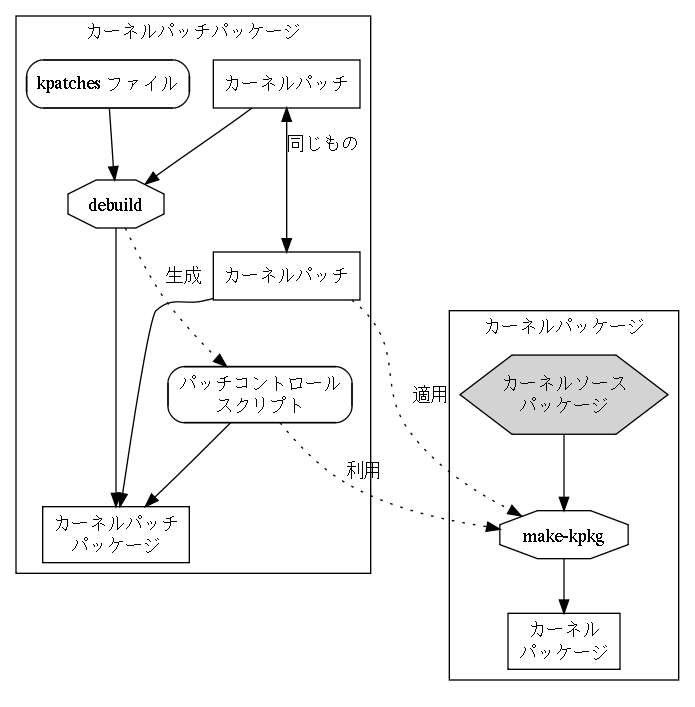
\includegraphics[width=0.8\hsize]{image200807/kpatch0.png}
 \end{center}
 \caption{Linux $B%+!<%M%k%Q%C%A(B $B$N(B Debian $B%Q%C%1!<%8$N;EAH$_(B}
 \label{fig:kpatch0}
\end{figure}

\subsection{$B%Q%C%1!<%8:n@.A0$N=`Hw(B}

\subsubsection{dh-kpatches $B%Q%C%1!<%8$N%$%s%9%H!<%k(B}
make-kpkg $B$,MxMQ$G$-$k(B Linux $B%+!<%M%k%Q%C%A%Q%C%1!<%8$r:n@.$9$k$K$O!"(Bdh-kpatches $B%Q%C%1!<%8$,I,MW$G$9!#(B
dh-kpatches $B$r;H$C$F!"%Q%C%1!<%82=(B
$B$r9T$&$3$H$K$h$j!"(Bkenrel-package $B$GDs6!$5$l$F$$$k(B make-kpkg $B%3%^%s%I$G%+!<%M%k%Q%C%A%Q%C%1!<%8$GDs6!$7$F$$$k(B
$B%Q%C%A$rE,MQ$7$?(B Linux $B%+!<%M%k%Q%C%1!<%8$,:n@.$G$-$k$h$&$K$J$j$^$9!#(B
$B%Q%C%1!<%8:n@.%5%]!<%HMQ$H$7$F!"(Bdh-make $B$r%$%s%9%H!<%k$7$F$*$/$HNI$$$G$7$g$&!#(Bdh-make $B$r;H$&$3$H$K$h$C$F!"%Q%C%1!<%8$N(B
$B?w7A$rMF0W$K:n@.$9$k$3$H$,$G$-$^$9!#(B
\begin{commandline}
$ sudo apt-get update
$ sudo apt-get install dh-kpatches dh-make build-essential
\end{commandline}

\subsubsection{$B%Q%C%A$NMQ0U(B}
$B$^$:!"%+!<%M%k8~$1$N%Q%C%A$r:n@.$9$kI,MW$,$"$j$^$9!#3+H/<T$K$h$C$F$O!"4{$K%Q%C%A$,%+!<%M%k%P!<%8%g%sKh$KMQ0U$5$l$F$$$k;v$b$"$j$^$9$,!"(B
$B:G6a$G$O!"(BLinus $B$N%D%j!<$KMF0W$KDI=>$G$-$k$h$&$K!"(BGit$B$r;H$C$F%=!<%9%3!<%I$,4IM}$5$l$F$$$k>l9g$,B?$$$G$9!#(B
POHMELFS $B$G$b(B $B%=!<%9%3!<%I$O(B Git $B$G4IM}$5$l$F$*$j!"0BDjHG$N%+!<%M%k!J$3$N869F$r=q$$$F$$$k;~E@$G$O!"(BLinux 2.6.25$B!K$K>o$KDI=>$5$l$F$$$^$9!#(B
$B$3$N:9J,$r<hF@$9$k$K$O!"(BGit $B%j%]%8%H%j$r<hF@$7!"(Bgit diff $B%3%^%s%IEy$G<h$j=P$;$P$h$$$G$7$g$&!#(B

\begin{commandline}
$ git clone http://tservice.net.ru/~s0mbre/archive/pohmelfs/pohmelfs.git
Initialized empty Git repository in /tmp/pohmelfs/.git/
got 37e1b82c0535386cf09b3821dff5e8cb5f9e26b4
walk 37e1b82c0535386cf09b3821dff5e8cb5f9e26b4
<snip>
$ cd pohmelfs
$ git tag
<snip>
v2.6.24-rc8
v2.6.25
v2.6.25-rc1
v2.6.25-rc2
<snip>
$ git diff v2.6.25 > ~/pohmelfs.diff
\end{commandline}

\subsubsection{$B%G%#%l%/%H%j$N:n@.(B}

$B%Q%C%A$,:n@.$G$-$?$i!"%Q%C%1!<%8:n@.MQ$N%G%#%l%/%H%j$r:n@.$7!"$=$NCf$K%Q%C%A%U%!%$%k$r%3%T!<$7$^$9!#(B
$B%G%#%l%/%H%jL>$O(B Debian$B$N%]%j%7!<$K9g$o$;$?$b$N(B($B%=%U%H%&%'%"$^$?$O5!G=L>(B-$B%P!<%8%g%s(B)$B$K$7$F$*$-!"%Q%C%A%U%!%$%kL>$O(B
$B%Q%C%A5!G=L>(B-$B%+!<%M%k%P!<%8%g%s(B $B$K$7$F$*$-$^$9!#$3$l$O!"$3$N$h$&$J%U%!%$%kL>$r(B dh-kpatches $B$,MW5a$9$k$?$a$G$9!#(B

\begin{commandline}
$ mkdir linux-patch-pohmelfs-20080707
$ cd linux-patch-pohmelfs-20080707
$ cp ../pohmelfs.diff pohmelfs-2.6.x
\end{commandline}

\subsection{dh\_make $B$r;H$C$??w7A$N:n@.(B}
$B%Q%C%1!<%8:n@.$N=`Hw$,$G$-$?$i!"(B dh\_make $B%3%^%s%I$r;H$C$F?w7A$r:n@.$7$^$9!#(B
dh\_make $B$K$O%+!<%M%k%Q%C%AMQ$N%5%]!<%H$O$J$$$N$G!"(Bsingle$B%P%$%J%j$N?w7A$r:n@.$9$k(B
$B%*%W%7%g%s$r;XDj$7$F!":n@.$7$^$9!#(B-r $B%*%W%7%g%s$O(B orig.tar.gz $B%U%!%$%k$r:n@.$7!"(B-s $B%*%W%7%g%s$O(B
$B%7%s%0%k%P%$%J%jMQ$N?w7A$r=PNO$7$^$9!#(B
\begin{commandline}
$ dh_make -r -s
Maintainer name : Nobuhiro Iwamatsu
Email-Address   : iwamatsu@nigauri.org 
Date            : Mon, 07 Jul 2008 01:00:33 +0900
Package Name    : linux-patch-pohmelfs
Version         : 20080707
License         : blank
Using dpatch    : no
Type of Package : Single
Hit <enter> to confirm: 
Currently there is no top level Makefile. This may require additional tuning.
Done. Please edit the files in the debian/ subdirectory now. You should also
check that the linux-patch-pohmelfs Makefiles install into $DESTDIR and not in / . 
\end{commandline}

\subsection{debian$B%G%#%l%/%H%jFb$NJQ99(B}
dh\_make $B%3%^%s%I$G(B $B%+!<%M%k%Q%C%A$r(B Debian $B%Q%C%1!<%8$K$9$k$?$a$N?w7A$,:n@.$G$-$^$7$?!#(B
$B$3$l$r85$KFbMF$rJQ99$7$F$$$-$^$9!#(B

\subsubsection{$B%5%s%W%k%9%/%j%W%HEy$N:o=|(B}
dh\_make $B$G:n@.$5$l$k%5%s%W%k%9%/%j%W%H$OI,MW$J$$$N$GA4$F:o=|$7$^$9!#(B
$B$^$?!"(B dirs $B%U%!%$%k$d(B doc $B%U%!%$%k$bI,MW$J$$$?$a:o=|$7$^$9!#(B
\begin{commandline}
$ rm -rf ./debian/*.ex ./debian/*.EX ./debian/doc ./debian/dirs
\end{commandline}

\subsubsection{debian/copyright $B$N=$@5(B}
$B%Q%C%A$N>pJs$K9g$o$;$F!"(Bdebiab/copyright $B$N=$@5$r9T$$$^$9!#(B
pohmelfs $B$N>l9g$O0J2<$N$h$&$K=$@5$7$^$9!#(B

\begin{commandline}
This package was debianized by Nobuhiro Iwamatsu <iwamatsu@nigauri.org> on
Mon, 07 Jul 2008 01:00:33 +0900.

It was downloaded from
        http://tservice.net.ru/~s0mbre/archive/pohmelfs/pohmelfs.git
This is Git repository. I made the difference of the latest committing a
patch from v2.6.25 tag.

Upstream Author(s):

    Evgeniy Polyakov <johnpol@2ka.mipt.ru>

Copyright:

    Copyright (C) 2008 Evgeniy Polyakov <johnpol@2ka.mipt.ru>

License:

 GPLv2

The Debian packaging is (C) 2008, Nobuhiro Iwamatsu <iwamatsu@nigauri.org> and
is licensed under the GPL, see `/usr/share/common-licenses/GPL'.

# Please also look if there are files or directories which have a
# different copyright/license attached and list them here.

\end{commandline}

\subsubsection{debian/README.Debian $B$N=$@5(B}
debain/README.Debian $B%U%!%$%k$K(B Debian $B$G;H$&$?$a$N(B HowTo$B$J$I$r=q$$$F$*$-$^$7$g$&!#(B
$B%5%]!<%H$7$F$$$k%+!<%M%k%P!<%8%g%s$d!"%+!<%M%k%$%a!<%8$N:n@.J}K!$J$I$r=q$$$F$*$/$N$,0lHLE*(B
$B$J$h$&$G$9!#(B

\begin{commandline}
linux-patch-pohmelfs for Debian
-------------------------------

This patch is pohmelfs support patch for Debian Linux kernel. 
You can try with linux-source-2.6.25 package. 

- How to use
  $ sudo apt-get install linux-source-2.6.25 libncurses-dev kernel-package
  $ cd /usr/src ; tar -xjf linux-source-2.6.25.tar.bz2 ; cd linux-source-2.6.25
  $ make-kpkg clean
  $ cp /boot/config-2.6.25-2-686 .config
  $ make menuconfig
  $ make-kpkg --rootcmd fakeroot --append-to-version -pohmelfs --revision 0.1 -added_patches=pohmelfs kernel-image

 -- Nobuhiro Iwamatsu <iwamatsu@nigauri.org>  Mon, 07 Jul 2008 01:00:33 +0900

\end{commandline}

\subsubsection{debian/control $B$N=$@5(B}
$B<!$K(B debian/control $B%U%!%$%k$r=$@5$7$^$9!#(B
$BCmL\$9$Y$-$H$3$m$O!":n@.$5$l$k%Q%C%1!<%8$G;XDj$7$F$"$k!"(B{\bf Depends: \$\{kpatch:Depends\}}$B$G$9!#(B
$B$3$3$G(B kpatch:Depends $B$r;XDj$9$k$3$H$K$h$C$F!"%+!<%M%k%Q%C%A%Q%C%1!<%8$r;H$C$?(B
$B%+!<%M%k:n@.$KI,MW$J0MB8%Q%C%1!<%8$rCV$-49$($F$/$l$^$9!#(B
$B$^$?!"%=!<%9%Q%C%1!<%8$N(B {\bf$B!!(BBuild-Depends}$B!!$K(B {\bf dh-kpatches$B!!%Q%C%1!<%8(B} $B$rDI2C$9$k;v$rK:$l$J$$$h$&$K$7$^$7$g$&!#(B

\begin{commandline}
Source: linux-patch-pohmelfs
Section: devel
Priority: extra
Maintainer: Nobuhiro Iwamatsu <iwamatsu@nigauri.org>
Build-Depends: debhelper (>= 6), dh-kpatches
Standards-Version: 3.8.0.1
Homepage: http://tservice.net.ru/~s0mbre/old/?section=projects&item=pohmelfs

Package: linux-patch-pohmelfs
Architecture: all
Depends: ${kpatch:Depends}
Description: POHMELFS kernel patch
 POHMELFS stands for Parallel Optimized Host Message Exchange Layered File System.
 Development status can be tracked in filesystem section.
 This is a high performance network filesystem with local coherent cache of data
 and metadata.
 Its main goal is distributed parallel processing of data. Network filesystem is a
 client transport.
 POHMELFS protocol was proven to be superior to NFS in lots (if not all, then it
 is in a roadmap) operations.
\end{commandline}

\subsubsection{debian/changelog $B$N=$@5(B}
dch $B%3%^%s%I$r;H$C$F(B debian/changelog $B%U%!%$%k$r=$@5$7$^$9!#(B
\begin{commandline}
$ dch
linux-patch-pohmelfs (20080707-1) unstable; urgency=low

  * Initial release                                          

 -- Nobuhiro Iwamatsu <iwamatsu@nigauri.org>  Mon, 07 Jul 2008 01:25:37 +090
\end{commandline}

\subsubsection{kpatches $B%U%!%$%k(B}

$B$I$N%Q%C%1!<%8Fb$K<}O?$5$l$F$$$k%Q%C%A$r$I$N%+!<%M%k%P!<%8%g%s$KEv$F$l$P$$$$$N$+$J$I$N(B
$B%3%s%H%m!<%k$9$k$?$a$N%U%!%$%k(B kpatches $B$rMQ0U$9$kI,MW$,$"$j$^$9!#(B
$B$3$N%U%!%$%k$O0J2<$N$h$&$J%U%)!<%^%C%H$K$J$C$F$*$j!"(B
$B%+!<%M%k%P!<%8%g%sKh$K(B Patch-file $B$H(B Kernel-version $B$N9`L\$rDI2C$9$kI,MW$,$"$j$^$9!#(B

\begin{commandline}
Patch-name: POHMELFS patch
Patch-id: pohmelfs <-- make-kpkg $B$N(B --added-patches $B$G;XDj$9$k%Q%C%AL>(B 
Architecture: all <-- $B%5%]!<%H$9$k%"!<%-%F%/%A%c(B
Path-strip-level: 1

Patch-file: pohmelfs-2.6.x <-- $B%Q%C%A%U%!%$%kL>(B
Kernel-version: 2.6.25 <-- $B%Q%C%A$,%5%]!<%H$9$k%+!<%M%k%P!<%8%g%s(B
\end{commandline}

\subsubsection{debian/rules $B%U%!%$%k$N=$@5(B}
debian/rules $B%U%!%$%k$GCm0U$9$kE@$H$7$F!"(B install $B%?!<%2%C%H$G!"(B
dh\_installkpatches $B$r;XDj$9$kI,MW$,$"$j$^$9!#(Bdh\_installkpatches $B$G(B
$B%+!<%M%k%Q%C%A$,(B kpatches $B%U%!%$%k$H6&$K$K%Q%C%1!<%8:n@.MQ$N0l;~%G%#%l%/%H%j$K%3%T!<$5$l$^$9!#(B

\begin{commandline}
#!/usr/bin/make -f

build: build-stamp
build-stamp:
        dh_testdir
        touch build-stamp

clean:
        dh_testdir
        dh_testroot
        rm -f build-stamp
        dh_clean

install: build
        dh_testdir
        dh_testroot
        dh_clean -k
        dh_installdirs
        dh_installkpatches

# Build architecture-independent files here.
binary-indep: build install
        dh_testdir
        dh_testroot
        dh_installchangelogs
        dh_link
        dh_strip
        dh_compress
        dh_fixperms
        dh_installdeb
        dh_shlibdeps
        dh_gencontrol
        dh_md5sums
        dh_builddeb

# Build architecture-dependent files here.
binary-arch: binary-indep

# We have nothing to do by default.

binary: binary-indep binary-arch
\end{commandline}

\subsection{$B%Q%C%1!<%8$N%S%k%I$*$h$S%$%s%9%H!<%k(B}
$B%Q%C%1!<%8$N%S%k%I$r9T$&:]$K$O!"DL>o$N%Q%C%1!<%8:n@.$HJQ$o$j$^$;$s!#(B
debuild $B$J$I$r;H$C$F%Q%C%1!<%8$N:n@.$r9T$C$F$/$@$5$$!#(B
$B:n@.$5$l$?%Q%C%1!<%8$r%$%s%9%H!<%k$9$k$H!"(B{\bf /usr/src/kernel-patches} $B$K%Q%C%A$H@)8fMQ$N%9%/%j%W%H$,(B
$B%$%s%9%H!<%k$5$l$^$9!#(Bmake-kpkg $B%3%^%s%I$O$3$N%G%#%l%/%H%j$r;2>H$7!"%Q%C%A$rE,MQ$7$^$9!#(B
\begin{commandline}
% debuild
% sudo dpkg -i ../linux-patch-pohmelfs_20080707-1_all.deb
\end{commandline}

\subsection{$B%Q%C%1!<%8$N%F%9%H(B}
$B%+!<%M%k%Q%C%A%Q%C%1!<%8$N%F%9%H$O!"%+!<%M%k%=!<%9%3!<%I$K(B
$B%Q%C%A$rEv$F!"%+!<%M%k$,%3%s%Q%$%k$G$-$k$+!"3NG'$9$kI,MW$,$"$j$^$9!#(B
$B$^$?!"(BDebian $B$N>l9g$O!"(BDebian $B$H(B kernel.org $B$GG[I[$7$F$$$k%+!<%M%k$N(B2$B<oN`$r9MN8$9$kI,MW$,$"$j$^$9$,!"(B
$BA0<T$NJ}$r%F%9%H$7$F$$$l$P==J,$G$7$g$&!#(B
$B%$%s%9%H!<%k$7$?%+!<%M%k%Q%C%A%Q%C%1!<%8$r;H$C$F!"%+!<%M%k$r%3%s%Q%$%k$9$k$K$O!"(B
make-kpkg $B%3%^%s%I$N(B--added\_patches $B$N%*%W%7%g%s$r;H$C$F!"%Q%C%A$r;XDj$7$^$9!#(B
$B%Q%C%A$,Ev$?$C$F$$$k$+%=!<%9$r3NG'$7!"%+!<%M%k$N%3%s%Q%$%k$,@5>o$K9T$o$l$F$$$k$+3NG'$7$^$7$g$&!#(B
$B$^$?!":n@.$5$l$?(B $B%+!<%M%k%Q%C%1!<%8$r<B:]$K%$%s%9%H!<%k$7!"%F%9%H$r9T$&$3$H$b=EMW$G$9!#(B

\begin{commandline}
$ sudo apt-get install linux-source-2.6.25 libncurses-dev kernel-package
$ cd /usr/src ; tar -xjf linux-source-2.6.25.tar.bz2 ; cd linux-source-2.6.25
$ make-kpkg clean
$ cp /boot/config-2.6.25-2-686 .config
$ make menuconfig
$ make-kpkg --rootcmd fakeroot --append-to-version -pohmelfs --revision 0.1 -added_patches=pohmelfs kernel-image
\end{commandline}

\subsection{$B%Q%C%1!<%8$N%"%C%W%G!<%HJ}K!(B}
$B$$$^$N$H$3$m!"%+!<%M%k%Q%C%A%=!<%9%Q%C%1!<%8$N%"%C%W%G!<%HJ}K!$,7h$^$C$F$$$^$;$s!#(B
$BE,Ev$J%G%#%l%/%H%j$r:n@.$7$F!"(Buupdate $B%3%^%s%I$r<B9T$9$k$N$,0lHVMF0W$H;W$o$l$^$9!#(B
$B>-MhE*$K$O!"%Q%C%A$r;XDj$9$k$3$H$K$h$C$F!"%=!<%9%Q%C%1!<%8$r%"%C%W%G!<%H$G$-$k$h$&$K(B
$B$7$?$$$H9M$($F$$$^$9!#(B

\subsection{$B$^$H$a(B}
$B0J>e$N<j=g$r;H$&$H!"(BLinux $B%+!<%M%k%Q%C%A$N(B Debian $B%Q%C%1!<%8$r:n@.$9$k$3$H$,$G$-$^$9!#(B
$B$7$+$7!"$3$N$^$^$G$O$+$J$j<j4V$,$+$+$j$^$9$N$G!":#2s$N@.2LJ*$r$^$H$a!"(B
dh-make $B$G(B Linux $B%+!<%M%k%Q%C%A%Q%C%1!<%8$N?w7A$,:n@.$G$-$k$h$&$K5!G=$rDI2C$7$^$7$?(B(\#304688)$B!#(B
$B$3$N%Q%C%A$,<h$j9~$^$l$k$H!"(Bdh-make $B$r;H$&$3$H$K$h$j!"$h$j4JC1$K(B Linux $B%+!<%M%k%Q%C%A%Q%C%1!<%8(B
$B$,:n@.$G$-$k$h$&$K$J$k$G$7$g$&!#(B
$B$A$J$_$K!"(Bpohmelfs $B$O(B linux-2.6.27 or 2.6.28 $B$K<h$j9~$^$l$k$h$&$G$9!#$h$+$C$?$h$+$C$?!#(B

\dancersection{Linux $B%+!<%M%k%b%8%e!<%k$N(B Debian $B%Q%C%1!<%8:n@.(B}{$B4d>>(B $B?.MN(B}
\label{sec:kmod}
\index{kmod}

\subsection{$B$O$8$a$K(B}
$B:#2s$O(B video $B%G!<%?(Bloopback $BMQ(B Linux $B%+!<%M%k%b%8%e!<%k!"(Bvloopback $B$rBj:`$K$7$F!"(B
Linux $B%+!<%M%k%b%8%e!<%k$N(B Debian $B%Q%C%1!<%8:n@.J}K!$r@bL@$7$^$9!#(B

\subsection{$B$J$<%+!<%M%k%b%8%e!<%k%=!<%9%3!<%I$r%Q%C%1!<%82=$9$k$N$+(B}
Linux $B$N(B $B%+!<%M%k%b%8%e!<%k%=!<%9%3!<%I$r%Q%C%1!<%82=$9$kM}M3$N0l$D$H$7$F!"(B
$B%+!<%M%k%P!<%8%g%s$K9g$o$;$?%I%i%$%P$r4IM}$9$k<j4V$,>J$1$k;v$H(B
$B%b%8%e!<%k%I%i%$%P%3%s%Q%$%k%U%m%s%H%(%s%I(B module-assistant 
$B$K$h$k(B $BA`:n$N$7$d$9$5$,Bg$-$$$G$7$g$&!#$3$N%=%U%H%&%'%"$r;H$&$3$H$K$h$C$F!"(B
$BMF0W$K%b%8%e!<%k$N%3%s%Q%$%k$*$h$S%$%s%9%H!<%k$r9T$&;v$,$G$-$^$9!#(B
$B8=;~E@$G$O!"%+!<%M%k%P!<%8%g%s$,>e$,$kEY$K%3%s%Q%$%k$9$kI,MW$,$"$j$^$9$,!"(B
$B%Q%C%1!<%82=$7$F$*$/$H!"$"$kDxEY$^$G<+F02=$G$-$k$?$a!"%"%C%W%G!<%H$bMF0W$K$J$j$^$9!#(B

\subsection{$B%+!<%M%k%b%8%e!<%k%Q%C%1!<%8$N;EAH$_(B}
$B%Q%C%1!<%8$N:n$jJ}$N@bL@$NA0$K%+!<%M%k%b%8%e!<%k%Q%C%1!<%8$N;EAH$_$K$D$$$F@bL@$7$^$9(B($B?^(B\ref{fig:mod0})$B!#(B
$B%+!<%M%k%b%8%e!<%k%Q%C%1!<%8$O(B $BFbIt$K(B $B%+!<%M%k%b%8%e!<%k%=!<%9%3!<%I$H%3%s%Q%$%k$9$k$?$a$N(B Makefile(debian/rules)
$B$H!"(Bcontrol $B%U%!%$%k(B(debian/control $B$KAjEv$9$k$b$N(B)$B$r8G$a$?$b$N$G$"$k(B $B%I%i%$%P%=!<%9%$%a!<%8$r;}$C$F$$$^$9(B $B!#(B
$B$3$N%I%i%$%P%=!<%9%$%a!<%8$O!"<B:]$O(B Debian $B%=!<%9%Q%C%1!<%8$H9=@.$OF1$8$K$J$C$F$*$j!"(B bzip2 $B$G05=L$7$?$b$N$K$J$j$^$9!#(B 
$B%+!<%M%k%b%8%e!<%k%Q%C%1!<%8$r%$%s%9%H!<%k$9$k$H!"(B/usr/src/$B$K(B $B%I%i%$%P%=!<%9%$%a!<%8$,CV$+$l!"(Bmodule-assistant $B$,(B
$B$3$N%U%!%$%k$r(B/usr/src/modules $B%G%#%l%/%H%j0J2<!"%S%k%IKh$KE83+$7!"%I%i%$%PMQ$N(B Debian $B%Q%C%1!<%8%S%k%I$r9T$$$^$9!#(B
$B:n@.$5$l$?(B $B%Q%C%1!<%8$O(B /usr/src $B$KCV$+$l$^$9!#(B
$B%b%8%e!<%k%=!<%9%Q%C%1!<%8$O!"$3$N%I%i%$%P%=!<%9%$%a!<%8$r:n@.$7!"(Bmodule-assistant $B$HO"7H$G$-$k5!G=$r(B
$BDs6!$7$^$9!#(B

\begin{figure}[h]
 \begin{center}
  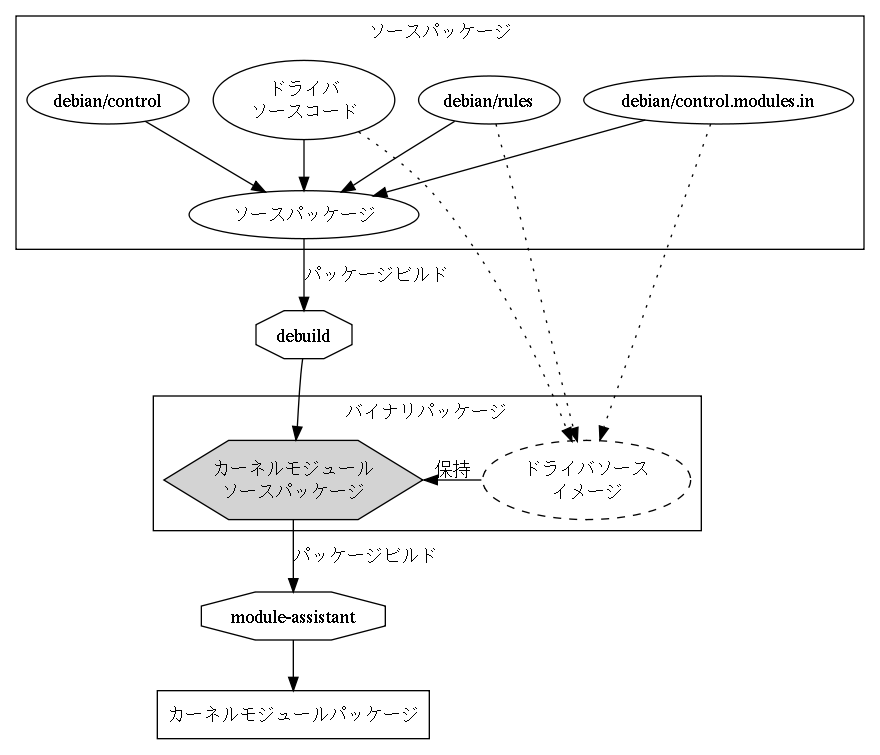
\includegraphics[width=0.8\hsize]{image200807/kmod0.png}
 \end{center}
 \caption{$B%+!<%M%k%b%8%e!<%k%Q%C%1!<%8$N;EAH$_(B}
 \label{fig:mod0}
\end{figure}

\subsection{$B%I%i%$%P%=!<%9%3!<%I$N<hF@$HE83+(B}
vloopback $B$O(B flashcam $B$H$$$&(B $B%U%j!<%=%U%H%&%'%"$H6&$KDs6!$5$l$F$$$^$9!#(B
$B:#2s$O!"(Bvloopback $B$N%=!<%9%3!<%I$@$1$r%?!<%2%C%H$K$9$k$N$G!"%=!<%9%3!<%I$r(B
$B<h$j=P$7$^$9!#(B
\begin{commandline}
$ wget http://www.swift-tools.net/Flashcam/flashcam-1.1.tgz
$ tar -xzf flashcam-1.1.tgz
$ cp -rf flashcam-1.1/vloopback-1.1.2 .
$ cd loopback-1.1.2
\end{commandline}

\subsection{dh\_make $B$r;H$C$??w7A$N:n@.(B}
$B%Q%C%1!<%8:n@.$N=`Hw$,$G$-$?$i!"(B dh\_make $B%3%^%s%I$r;H$C$F?w7A$r:n@.$7$^$9!#(B
dh\_make $B$K$O!"%+!<%M%k%b%8%e!<%k$N?w7A$r:n@.$9$k%*%W%7%g%s(B -k / --kmod $B$,Ds6!$5$l$F$$$^$9!#(B

\begin{commandline}
$ dh_make -k -r 
Maintainer name : Nobuhiro Iwamatsu
Email-Address   : iwamatsu@nigauri.org 
Date            : Tue, 15 Jul 2008 23:21:23 +0900
Package Name    : vloopback
Version         : 1.1.2
License         : blank
Using dpatch    : no
Type of Package : Kernel Module
Hit <enter> to confirm: 
Done. Please edit the files in the debian/ subdirectory now. You should also
check that the vloopback Makefiles install into $DESTDIR and not in / .
\end{commandline}

\subsection{debian$B%G%#%l%/%H%jFb$NJQ99(B}
Debian $B%Q%C%1!<%8$K$9$k$?$a$N?w7A$,:n@.$G$-$?$N$G!"$3$l$r85$KFbMF$rJQ99$7$F$$$-$^$9!#(B

\subsubsection{$B%5%s%W%k%9%/%j%W%HEy$N:o=|(B}
dh\_make $B$G:n@.$5$l$k%5%s%W%k%9%/%j%W%H$OI,MW$J$$$N$GA4$F:o=|$7$^$9!#(B
\begin{commandline}
$ rm -rf ./debian/*.ex ./debian/*.EX
\end{commandline}

\subsubsection{debian/copyright $B$N=$@5(B}
$B%Q%C%A$N>pJs$K9g$o$;$F!"(Bdebiab/copyright $B$N=$@5$r9T$$$^$9!#(B
vloopback $B$N>l9g$O0J2<$N$h$&$K=$@5$7$^$9!#(B

\begin{commandline}
This package was debianized by Nobuhiro Iwamatsu <iwamatsu@nigauri.org> on
Tue, 15 Jul 2008 23:21:23 +0900.

It was downloaded from <http://www.swift-tools.net/Flashcam/flashcam-1.1.tgz>

Upstream Author(s):

    Olivier Debon <olivier@debon.net>

Copyright:

    Copyright (C) 2008 Olivier Debon <olivier@debon.net>

License:

    GPLv2

The Debian packaging is (C) 2008, Nobuhiro Iwamatsu <iwamatsu@nigauri.org> and
is licensed under the GPL, see `/usr/share/common-licenses/GPL'.

# Please also look if there are files or directories which have a
# different copyright/license attached and list them here.
\end{commandline}

\subsubsection{debian/README.Debian $B$N=$@5(B}
debain/README.Debian $B%U%!%$%k$r=$@5$7$^$9!#(B
$B?w7A$,$"$kDxEY=q$$$F$*$$$F$/$l$F$$$k$N$G!"$"$^$j=$@5$9$kI,MW$O$"$j$^$;$s!#(B
$B3NG'$7$?(B Linux $B%+!<%M%k%P!<%8%g%s$J$I$r=q$$$F$*$/$HNI$$$+$b$7$l$^$;$s!#(B

\begin{commandline}
vloopback for Debian
--------------------

Please see ./README for a description of the vloopback software.

The Debian vloopback source package provides two packages,

 vloopback-source, which provides the source for the kernel modules

The vloopback-source package can be used in several ways,

 - Using the make-kpkg(1) command provided by the kernel-package Debian
   package. This will produce a corresponding vloopback-modules package for
   the Debian kernel-image package that you are using. This is "the Debian
   way". See the "modules_image" section of the make-kpkg(1) man page.

 - Changing to the /usr/src/modules/vloopback/ directory and building as
   the README file instructs using "make; make install". This will build
   and install a module specific to the system you are building on and is
   not under control of the packaging system.

 -- Nobuhiro Iwamatsu <iwamatsu@nigauri.org>  Tue, 15 Jul 2008 23:21:23 +0900
\end{commandline}

\subsubsection{debian/control $B$N=$@5(B}
$B<!$K(B debian/control $B%U%!%$%k$r=$@5$7$^$9!#(B
dh\_make $B$G:n@.$7$?>l9g$O!"(Bvloopback-utils $B$H$$$C$?!"%I%i%$%P$r%5%]!<%H$9$k$?$a$N(B
$B%Q%C%1!<%8$r:n@.$9$k%(%s%H%j$,$"$j$^$9!#(B
$B%=!<%9%3!<%I$K%D!<%k$,4^$^$l$F$$$k>l9g$O!"$3$N%(%s%H%j$r;H$C$F!"%D!<%kMQ$N%Q%C%1!<%8$r(B
$B:n@.$G$-$k$h$&$K$J$C$F$$$^$9!#:#2s$OI,MW$J$$$N$G:o=|$7$^$9!#(B

\begin{commandline}
Source: vloopback
Section: graphics
Priority: extra
Maintainer: Nobuhiro Iwamatsu <iwamatsu@nigauri.org>
Build-Depends: debhelper (>= 7), bzip2
Standards-Version: 3.8.0.1
Homepage: http://www.swift-tools.net/Flashcam/

Package: vloopback-source
Architecture: all
Depends: module-assistant, debhelper (>= 7), make, bzip2
Description: Source for the vloopback driver.
 This package provides the source code for the vloopback kernel modules.
 The vloopback package is also required in order to make use of these
 modules. Kernel source or headers are required to compile these modules.
\end{commandline}

\subsubsection{debian/changelog $B$N=$@5(B}
dch $B%3%^%s%I$r;H$C$F(B debian/changelog $B%U%!%$%k$r=$@5$7$^$9!#(B
\begin{commandline}
$ dch
vloopback (1.1.2-1) unstable; urgency=low

  * Initial release

 -- Nobuhiro Iwamatsu <iwamatsu@nigauri.org>  Tue, 15 Jul 2008 23:21:23 +0900
\end{commandline}

\subsubsection{control.modules.in $B%U%!%$%k$N=$@5(B}
$B%+!<%M%k%b%8%e!<%k%=!<%9%Q%C%1!<%8$O!!(B2$B$D$N(B control $B%U%!%$%k$r;}$A$^$9!#(B
$B0l$D$O!"%+!<%M%k%b%8%e!<%k%=!<%9%Q%C%1!<%8MQ!"$b$&0l$D$O(B $B%+!<%M%k%b%8%e!<%k%Q%C%1!<%8MQ$N(B
$B%+!<%M%k%b%8%e!<%k%=!<%9%Q%C%1!<%8(B $BMQ$N(B debian/contorl $B%U%!%$%k$,(B control.modules.in $B$G$9!#(B
$B%I%i%$%P%Q%C%1!<%8:n@.;~$K(B 
$B%=!<%9%Q%C%1!<%8$+$i%+!<%M%k%b%8%e!<%k%=!<%9%Q%C%1!<%8$,:n@.$5$l!"%f!<%6$O%+!<%M%k%b%8%e!<%k%=!<%9%Q%C%1!<%8(B
$B$r%3%s%Q%$%k$7!"%+!<%M%k%b%8%e!<%k%Q%C%1!<%8$r:n@.$7!"%$%s%9%H!<%k$7$FMxMQ$7$^$9!#(B
$B$3$N%U%!%$%k$NCf$K$O%+!<%M%k$N%P!<%8%g%s$K$h$C$FCV49$5$l$kJ8;zNs$,(B \texttt{\_KVERS\_} $B$H$$$&J8;zNs$K$J$C$F$$$^$9!#(B
{\bf control.modules.in} $B$O(B {\bf module-assistant} $B$J$I$K$h$j=hM}$5$l!"(B
$B3F(BLinux $B%+!<%M%k%P!<%8%g%sMQ$NFbMF$KJQ99$5$l$^$9!#(B

\begin{commandline}
Source: vloopback
Section: graphics
Priority: optional
Maintainer: Nobuhiro Iwamatsu <iwamatsu@nigauri.org>
Build-Depends: debhelper (>= 7)
Standards-Version: 3.8.0.1

Package: vloopback-modules-_KVERS_
Architecture: any
Provides: vloopback-modules
Description: vloopback modules for Linux (kernel _KVERS_).
 This package contains the set of loadable kernel modules for the
 <description>.
 .
 This package contains the compiled kernel modules for _KVERS_
 .
 If you have compiled your own kernel, you will most likely need to build
 your own vloopback-modules. The vloopback-source package has been
 provided for use with the Debian's module-assistant or kernel-package
 utilities to produce a version of vloopback-modules for your kernel.
\end{commandline}

\subsubsection{debian/rules $B%U%!%$%k$N=$@5(B}

dh\_make $B$G:n@.$5$l$?!"(Bdebian/rules $B%U%!%$%k$O(B $B%Q%C%1!<%8:n@.MQ$N%?!<%2%C%H(B(build/install/clean)$B$H!"(B
$B%I%i%$%P%Q%C%1!<%8:n@.MQ$N%?!<%2%C%H(B binary-modules/kdist\_clean $B$,MQ0U$5$l$F$$$^$9!#(B
$B$3$l$i$N%?!<%2%C%H$NCf$r=$@5$7$^$9!#(B
\begin{commandline}
#!/usr/bin/make -f

psource:=vloopback-source
sname:=vloopback

# prefix of the target package name
PACKAGE=vloopback-modules
# modifieable for experiments or debugging m-a
MA_DIR ?= /usr/share/modass
# load generic variable handling
-include $(MA_DIR)/include/generic.make
# load default rules, including kdist, kdist_image, ...
-include $(MA_DIR)/include/common-rules.make

kdist_config: prep-deb-files
kdist_clean: clean
	$(MAKE) $(MFLAGS) -f debian/rules clean

configure: configure-stamp
configure-stamp:
	dh_testdir
	# Add here commands to configure the package.

	touch configure-stamp

build-arch: configure-stamp  build-arch-stamp
build-arch-stamp: 
	dh_testdir

	# Add here command to compile/build the package.
	# $(MAKE)

	touch $@

#k = $(shell echo $(KVERS) | grep -q ^2.6 && echo k)

# during a normal build
binary-modules:
	dh_testroot
	dh_clean -k
	dh_installdirs lib/modules/$(KVERS)/misc

	# Build the module
	$(MAKE) KVER=$(KVERS) KSRC=$(KSRC)

	# Install the module
	cp vlooopbackko debian/$(PKGNAME)/lib/modules/$(KVERS)/misc

	dh_installdocs
	dh_installchangelogs
	dh_compress
	dh_fixperms
	dh_installdeb
	dh_gencontrol -- -v$(VERSION)
	dh_md5sums
	dh_builddeb --destdir=$(DEB_DESTDIR)
	dh_clean -k
\end{commandline}

\begin{commandline}
build-indep:  configure-stamp build-indep-stamp
build-indep-stamp: 
	dh_testdir
	touch $@

build: build-arch build-indep

clean: 
	dh_testdir
	rm -f build-arch-stamp build-indep-stamp configure-stamp
	dh_clean

install: DH_OPTIONS=
install: build
	dh_testdir
	dh_testroot
	dh_clean -k
	dh_installdirs

	# Create the directories to install the source into
	dh_installdirs -p$(psource)  usr/src/modules/$(sname)/debian

	# Copy only the driver source to the proper location
	cp vloopback.c  debian/$(psource)/usr/src/modules/$(sname)/.
	# Copy the needed debian/ pieces to the proper location
	cp debian/*modules.in* \
		debian/$(psource)/usr/src/modules/$(sname)/debian
	cp debian/rules debian/changelog debian/copyright \
		debian/compat debian/$(psource)/usr/src/modules/$(sname)/debian/
	cd debian/$(psource)/usr/src && tar c modules | bzip2 -9 > $(sname).tar.bz2 && rm -rf modules

	# Add here commands to install the package into debian/vloopback.
	# $(MAKE) DESTDIR=$(CURDIR)/debian/vloopback install

	dh_install

# Build architecture-independent files here.
# Pass -i to all debhelper commands in this target to reduce clutter.
binary-indep: build install
	dh_testdir -i
	dh_testroot -i
	dh_installchangelogs  -i
	dh_installdocs -i
	dh_installexamples -i
	dh_installman -i
	dh_link -i
	dh_compress -i
	dh_fixperms -i
	dh_installdeb -i
	dh_gencontrol -i
	dh_md5sums -i
	dh_builddeb -i

# Build architecture-dependent files here.
binary-arch: build install
	dh_testdir -s
	dh_testroot -s
	dh_installdocs -s
	dh_installinfo -s
	dh_installchangelogs  -s
	dh_compress -s
	dh_fixperms -s
	dh_installdeb -s
	dh_shlibdeps -s
	dh_gencontrol -s
	dh_md5sums -s
	dh_builddeb -s

binary: binary-indep binary-arch
.PHONY: build clean binary-indep binary-arch binary install configure binary-modules kdist kdist_configure kdist_image kdist_clean

\end{commandline}

\subsection{$B%Q%C%1!<%8$N%S%k%I$*$h$S%$%s%9%H!<%k(B}
$B%Q%C%1!<%8$N%S%k%I$r9T$&:]$K$O!"DL>o$N%Q%C%1!<%8:n@.$HJQ$o$j$^$;$s!#(B
debuild $B$J$I$r;H$C$F%Q%C%1!<%8$N:n@.$r9T$C$F$/$@$5$$!#(B
$B:n@.$5$l$?%Q%C%1!<%8$r%$%s%9%H!<%k$9$k$H!"(B{\bf /usr/src/modules} $B$K%I%i%$%P%=!<%9%$%a!<%8$,(B
$B%$%s%9%H!<%k$5$l$^$9!#(B
\begin{commandline}
% debuild
% sudo dpkg -i ../vloopback-source_1.1.2-1_all.deb
\end{commandline}

\subsection{$B%b%8%e!<%k%Q%C%1!<%8$N:n@.(B}
\subsubsection{module-assistant$B$r;H$C$?%3%s%Q%$%k(B}
$B%I%i%$%P%Q%C%1!<%8$N%3%s%Q%$%k$K$O(B module-assistant $B%3%^%s%I$rMxMQ$7$^$9!#(B
$B$3$N%3%^%s%I$O(B GUI$B$r;}$C$F$*$j!"(BGUI$B$G%I%i%$%P$N%3%s%Q%$%k$d%3%s%Q%$%k4D6-$N(B
$B%"%C%W%G!<%H$r9T$&;v$,$G$-$^$9!#(B
GUI$B$GA*Br$G$-$k%I%i%$%P72$O(B module-assistat$B%Q%C%1!<%8Fb$G;}$C$F$$$k%j%9%H(B(/usr/share/modass/compliant.list)$B$N$_(B
$B$,BP>]$K$J$C$F$$$k$?$a!"?7$7$/:n@.$7$?$b$N$OA*Br$G$-$^$;$s!#(B
$B$3$N$h$&$J>l9g$O!"%b%8%e!<%kL>$r;XDj$9$k$3$H$K$h$C$F%3%s%Q%$%k2DG=$G$9!#(B
\begin{commandline}
$ sudo m-a build vloopback
Extracting the package tarball, /usr/src/vloopback.tar.bz2, please wait...
/usr/bin/make clean
make[1]: $B%G%#%l%/%H%j(B `/usr/src/modules/vloopback' $B$KF~$j$^$9(B

<snip>

make[3]: $B%G%#%l%/%H%j(B `/usr/src/linux-headers-2.6.25-2-686' $B$KF~$j$^$9(B
  CC [M]  /usr/src/modules/vloopback/vloopback.o
  Building modules, stage 2.
  MODPOST 1 modules
  CC      /usr/src/modules/vloopback/vloopback.mod.o
  LD [M]  /usr/src/modules/vloopback/vloopback.ko
make[3]: $B%G%#%l%/%H%j(B `/usr/src/linux-headers-2.6.25-2-686' $B$+$i=P$^$9(B
make[2]: $B%G%#%l%/%H%j(B `/usr/src/modules/vloopback' $B$+$i=P$^$9(B
# Install the module
cp vloopback.ko debian/vloopback-modules-2.6.25-2-686/lib/modules/2.6.25-2-686/misc
dh_installdocs
dh_installchangelogs
dh_compress
dh_fixperms
dh_installdeb
dh_gencontrol -- -v1.1.2-1+2.6.25-6
dh_md5sums
dh_builddeb --destdir=/usr/src
dpkg-deb: `/usr/src/vloopback-modules-2.6.25-2-686_1.1.2-1+2.6.25-6_i386.deb' $B$K%Q%C%1!<%8(B `vloopback-modules-2.6.25-2-686' $B$r9=C[$7$F$$$^$9!#(B
dh_clean -k

<snip>
\end{commandline}

\subsubsection{make-kpkg$B$r;H$C$?%3%s%Q%$%k(B}  
modules-assistant $B0J30$K$b(B make-kpkg $B$N(B --added-modules $B%*%W%7%g%s$r;H$&$3$H$K$h$C$F(B
$B%3%s%Q%$%k$9$k$3$H$,$G$-$^$9!#$7$+$7!"(Bmake-kpkg $B$N>l9g$K$O%i%$%P%=!<%9%$%a!<%8$rE83+$7$F$/$l$J$$(B
$B$N$G!"<jF0$GE83+$9$kI,MW$,$"$j$^$9!#(B
kernel-package $B$O%+!<%M%k%Q%C%1!<%8@lMQ$H9M$($?$[$&$,$h$5$=$&$G$9!#(B
$B!J$=$N$?$a$K(B modules-assistant $B$,$G$-$?$N$G!#!K(B

\subsection{$B$^$H$a(B}
$B:G6a$O%I%i%$%P$b(B linus $B%D%j!<$K<h$j9~$^$l$d$9$/$J$C$?$N$G!"Aa$/;H$$$?$$?M8~$1$N(B
$B%Q%C%1!<%8$K$J$j$D$D$"$k%I%i%$%P%Q%C%1!<%872$G$9$,!"%f!<%6$N;v$r9M$($k$H(B
$B=EMW$J%Q%C%1!<%8$K$J$C$F$$$k$H;W$$$^$9!#:#8e$O$3$l$i$N%Q%C%1!<%8$r$I$N$h$&$K(B
$B%Q%C%1!<%8$H$7$F%a%s%F%J%s%9$7$F$$$/$+$J$I$K$D$$$FD4$Y$F$$$3$&$H;W$$$^$9!#(B

\subsection{$B$*$^$1(B}
module-assistant $B$G%5%]!<%H$5$l$F$$$k%Q%C%1!<%8$,$I$l$0$i$$%3%s%Q%$%k$G$-$k$N$+D4$Y$F$_$^$7$?!#(B
$B%"!<%-%F%/%A%c$O(B i386 $B!"%G%#%9%H%j%S%e!<%7%g%s$O(B sid $B$G$9!#%Q%C%1!<%8$O(B /usr/share/modass/compliant.list $B$K$+$+$l$F$$$k$b$N$G$9!#(B
$B7k2L$O(B82$B8DCf!"%3%s%Q%$%k(BOK: 22/ $B%3%s%Q%$%k(BNG: 22/ $B%Q%C%1!<%8$J$7(B: 38 $B$K$J$j$^$7$?!#%Q%C%1!<%8$J$7$J$N$O!"(Bmodule-assistant $B$N%j%9%H$,%a%s%F%J%s%9$5$l$F$$$J$+$i$@$H;W$$$^$9!#$"$H$O!"%"!<%-%F%/%A%cHsBP1~$J$I!#(B
$B4{$K%+!<%M%k$K%^!<%8$5$l$F$$$k$b$N$,$1$C$3$&$"$j!"%3%s%Q%$%k%(%i!<$O3F%a%s%F%J$,%5%\$C$F$$$k$N$G$7$g$&!#(B
$B$3$l$i$O:#8e(BBTS$B$7$F$$$/$D$b$j$G$9!#(B
 
\clearpage


%===========================================================%
\begin{getsureiupdate}{$B7nNc(B Nexenta Operation System}{$B>e@n(B $B=c0l(B}
\index{Nexenta}
$B@h7n$K$D$E$$$F(BNexenta$B$r$$$8$C$F8+$?$N$G$*EA$($7$^$9!#(B

$B<BMQE*$J%"%W%j%1!<%7%g%s$r%S%k%I$9$k$^$G$KA02s$O;j$j$^$;$s$G$7$?!#(B
$B$=$3$G!":#2s$O(Bdlsym $B$r;H$C$F<+M3<+:_$K%i%$%V%i%j$r%m!<%I$G$-$k$h$&$K$7$F$_$k$H$3$m$+$i(B
 $B$^$:$d$C$F$_$^$7$g$&!#(B

dlsym$B$G%m!<%I$G$-$k:GDc8B$N6&M-%i%$%V%i%j$r:n@.$9$k$H$3$m$+$i;O$a$F$_$^(B
$B$7$g$&!#(B


$B$^$:!"4X?t0l$D$@$1$rDj5A$7$?(BC$B$N%U%!%$%k$+$i:GDc8B$N6&M-%i%$%V%i%j$r:n@.(B
 $B$7$F$_!"$=$l$r<B9T$9$k$@$1$N%W%m%0%i%`$H!"(Bdlopen$B7PM3$GMxMQ$9$k%W%m%0%i(B
 $B%`$r:n@.$7$F$_$^$7$?!#(B

\begin{commandline}
// a.c : $B%5%s%W%k$N6&M-%i%$%V%i%j$N%3!<%I(B
#include <stdio.h>

void func1 (int i)
{
  printf(" hello world %i\n", i);
}
\end{commandline}

\begin{commandline}
// use.c: $BDL>o$N6&M-%i%$%V%i%jMxMQ(B
#include <stdio.h>

void func1 (int i);

main()
{
  func1(1);
}
\end{commandline}

\begin{commandline}
// dlopen.c: dlopen$B$G$N%P%$%J%jMxMQ(B
#include <dlfcn.h>
static int (*myfunc1)(int i) = NULL;
int main()
{
  void* h=dlopen("./liba.so", RTLD_NOW);
  
  myfunc1=dlsym(h, "func1");
  
  myfunc1(10);
  
  return 0;
}
\end{commandline}

$B$3$l$i$r%3%s%Q%$%k!"%j%s%/$7$F$_$F!"F0:n$r3NG'$7$F$_$^$7$?!#(B
$B$I$&$d$i(BLinux$B$H$"$^$j$+$o$i$J$$$h$&$G$9!#(B

\begin{commandline}
 + gcc -shared a.c -o liba.so
 + gcc use.c ./liba.so -o use
 + ./use
 hello world 1
 + gcc dlopen.c -o dlopen
 + ./dlopen
 hello world 10
\end{commandline}

$B$?$@$7!"$3$l$@$1$@$H%P!<%8%g%s%7%s%\%k$rMxMQ$7$?>l9g$K(Bdlsym $B$G$O$I$N%P!<(B
 $B%8%g%s$rMxMQ$9$k$N$+$,;XDj$G$-$J$$$h$&$JJ70O5$$,$?$@$h$C$F$$$^$9!#(B
$B$H$$$&$H$3$m$^$G3NG'$7$?$H$3$m$G:#7n$bNO?T$-$^$7$?!#(B
$B$^$?Mh7nB3$-$r$J$,$a$F$_$^$7$g$&!#(B
$B$b$7$+$9$k$H%P!<%8%g%s%7%s%\%k$N:n@.$H$=$NMxMQ$r$9$k$+$b$7$l$^$;$s!#(B

\end{getsureiupdate}
%===========================================================%


%\printindex

\cleartooddpage

\vspace*{15cm}
\hrule
\vspace{2mm}

\includegraphics[width=2cm]{image200502/openlogo-nd.eps}
\noindent \Large \bf Debian $BJY6/2q;qNA(B\\ \\
\noindent \normalfont \debmtgyear{}$BG/(B\debmtgmonth{}$B7n(B\debmtgdate{}$BF|(B \hspace{5mm}  $B=iHGBh(B1$B:~H/9T(B\\
\noindent \normalfont $BEl5~%(%j%"(B Debian $BJY6/2q(B $B!JJT=8!&0u:~!&H/9T!K(B\\
\hrule


\end{document}
